\chapter[Supervised learning in software development]{New supervised learning approaches to software development}
\label{chap:dsselection}

This chapter is entirely original and it focuses on the problem of dynamically selecting, using supervised learning approaches, the most suitable representation for an abstract data type according to the software system's current execution context. In this direction, a neural network approach and a support vector machine approach are proposed. 

The supervised learning approaches for the problem of automatic selection of data representations presented  in this chapter are original works published in  \cite{Czibula11Intelligent} and under review in \cite{Czibula12SVM}.

Selecting and creating the appropriate data structure for implementing an abstract data type (ADT) can greatly impact the performance of a software system. It is not a trivial problem for a software developer, as it is hard to anticipate all the usage scenarios of the deployed application. It is not clear how to select a good implementation
for an abstract data type when access patterns to it are
highly variant, or even unpredictable. Due to this fact, the software system may choose the appropriate data representation, at runtime, based on the effective data usage pattern. This dynamic selection can be achieved using machine learning techniques, which can assure complex and adaptive systems development.

In this chapter we approach the problem of dynamically selecting, using supervised learning approaches, the most suitable representation for an abstract data type according to the software system's current execution context. In this direction, a neural network model and a support vector machine model are proposed. The considered problem arises from practical needs, it has a major importance for software developers. Improper use of data structures in software applications leads to performance degradation and high memory consumption. These problems can be avoided by properly selecting data structures for implementing ADTs, according to the nature of the manipulated data.

To our knowledge, so far, there are no existing machine learning approaches for the problem of automatic selection of data representations.

The chapter is structured as follows. In Section \ref{mot} the problem of dynamic data structure selection is presented. It is explained that this is a complex problem because each particular data structure is usually more efficient for some operations and less efficient for others and that is why a static analysis for choosing the best representation can be inappropriate, as the performed operations can not be statically predicted. A practical example is presented and an experiment is performed in order to motivate our approach. 
In Section \ref{our} we present our first proposal of using supervised learning for dynamically selecting the implementation of an abstract data type from the software system, based on its current execution context. For this purpose, a neural network model will be used. In fact, selecting the most appropriate implementation of an abstract data type is equivalent to predicting, based on the current execution context, the type and the number of operations performed on the ADT, on a certain execution scenario.
In Section \ref{exp} we evaluate the accuracy of the technique proposed in Section \ref{our}, i.e. the ANN model's prediction accuracy. Starting from a data set given at \cite{forina}, we have simulated an experiment for selecting the most appropriate data structure for implementing the $List$ ADT. Experimental results suggest that our approach provides optimized data structure selection and reduces the computational time by selecting the data structure implementation which provides a minimum overall complexity for the operations performed on a certain abstract data type on a given execution scenario. Section \ref{cmp} presents a comparison to related work.
In Section \ref{sec:drspsvm} the problem of data representation selection problem (DRSP) is approached using support vector machines. Computational experiments from Section \ref{compexp} confirm a good performance of the proposed model and indicates the potential of our proposal. The advantages of our approach in comparison with similar approaches are also emphasized in Section \ref{sec:cmpsvm}.  



The original contributions of this chapter are:

\begin{itemize}

\item To introduce a supervised learning approach for the dynamic selection of abstract data types implementations during the execution of a software system, in order to increase the system's efficiency (Section \ref{our}) \cite{Czibula11Intelligent, Czibula12SVM} . 

\item To approach the considered problem using neural networks (Section \ref{ann}) \cite{Czibula11Intelligent}.

\item To evaluate the accuracy of the proposed neural network based technique on a case study (Section \ref{exp}) \cite{Czibula11Intelligent}.

\item To approach the considered problem using support vector machines (Section \ref{sub:methodologysvm}) \cite{Czibula12SVM}.

\item To evaluate the accuracy of the proposed support vector machine based technique on a case study (Section \ref{compexp})  \cite{Czibula12SVM}.

\item To emphasize the advantages of the proposed supervised learning approaches to DRSP in comparison with existing similar approaches (Section \ref{cmp} and Section \ref{sec:cmpsvm}) \cite{Czibula11Intelligent, Czibula12SVM} .


\end{itemize}





\section{The problem of dynamic data structure selection}
\label{mot}


Abstract data types (ADTs) \cite{adt} are used in software applications to model real world entities from the application domain. An ADT can be implemented using different data structures. The study of data structures and the algorithms that manipulate them is among the most fundamental topics in computer science \cite{mount}. Most of what
computer systems spend their time doing is storing, accessing, and manipulating data in one form or another. There are numerous examples from all areas
of computer science where a relatively simple application of good data structure techniques resulted in massive savings in computation time and, hence, money.

Selecting and creating the appropriate data structure for implementing an abstract data type can greatly impact the performance of a software system.
It is not a trivial problem for a software developer, as it is hard to anticipate all the use scenarios of the deployed application. It is not clear how to select a good implementation
for an abstract data type when access patterns to it are
highly variant, or even unpredictable. Due to this fact, the software system may choose the appropriate data representation, at runtime, based on the effective data usage pattern. This dynamic selection can be achieved using machine learning techniques \cite{mitchell}, which can assure complex and adaptive systems development.

In this chapter we approach the problem of dynamically selecting, using a supervised learning approach, the most suitable representation for an abstract data type according to the software system's current execution context. In this direction, a neural network model is proposed. The considered problem arises from practical needs, it has a major importance for software developers. Improper use of data structures in software applications leads to performance degradation and improper memory consumption. These problems can be avoided by properly selecting data structures for implementing ADTs, according to the nature of the manipulated data.

To our knowledge, so far, there are no existing machine learning approaches for the problem of automatic selection of data representations.





We have chosen neural networks as a machine learning method, as we consider they are good non-linear classification models and they are useful in prediction processes. Neural networks are adaptive systems that change their structure based on the information flow. They have good accuracy and are tolerant to noisy data. Neural networks are well-suited for modelling complex relationships and for situations in which there is little knowledge between the attributes and the classes of a dataset. So, in our opinion neural networks are very good for predicting the most suitable implementation of an abstract data type.

The rest of the paper is structured as follows. Section \ref{mot} gives a motivation for our work.  Our supervised leaning approach for a dynamic identification of the most suitable implementation of an ADT is introduced in Section \ref{our}. Section \ref{exp} provides an  evaluation of the proposed model on a case study. Existing approaches in the direction of automatic selection of data representations are presented in Section \ref{cmp}. We also provide a comparison of our approach with other
similar existing approaches. Section
\ref{conc} contains some conclusions of our paper and future
research directions.




The primary justification for a data structure selection
approach is that finding good representations
has proven to be difficult. This is mainly due to a lack of awareness of the importance
of the proper choices for data structures, issue that has a major impact on software systems' performance.

Each software system use abstract data types \cite{adt} to model real world entities from the application domain. Because abstract data types represent the core for any software application, a proper use of them is an essential requirement for developing a robust and efficient system.  We are focusing in this paper on container abstract data types, such as: collections, sets, lists and maps \cite{Cormen09Introduction}.

The design and implementation of efficient abstract data types are important issues for software developers. An ADT provides a set of operations that can be performed on it (the ADT's \emph{interface}/\emph{contract}). There are several possible implementations for an ADT, each implementation has to satisfy the ADT's contract. Each possible implementation of an abstract data type uses certain representations (\emph{data structures}) for the elements within the ADT's domain. Thus, selecting and creating the appropriate data structure for implementing an abstract data type can greatly impact the performance of the system. It is not a trivial problem for a software developer, as it is hard to anticipate all the use scenarios of the deployed application. It is not clear how to select a good implementation
for an abstract data type when access patterns to it are
highly variant, or even unpredictable. Previous approaches rely on compile-time analyses or programmer annotations \cite{chuang}.

A common situation is where there are several data structures for implementing an ADT,
with one data structure more efficient than the others for
certain operations from the ADT's interface but worst for the remaining operations,
and vice versa \cite{chuang}. The problem is how to choose the most appropriate data structure for implementing the ADT,
given that there is no \emph{a priori} knowledge of what operations,
and how often, the ADT will be mostly used for?
This is known as the \emph{data representation selection problem} \cite{sch}, or \emph{data structure selection problem} \cite{31}.
The problem can be considered for built-in data types (such as List, Collection), as well for user-defined abstract data types which can be implemented with several data structures.

The problem of automatic data structure selection is a complex one because each particular data structure is usually more efficient for some operations and less efficient for others and that is why a static analysis for choosing the best representation can be inappropriate, as the performed operations can not be statically predicted.

A ``static'' approach in solving the above presented problem can be, for example, to design a data structure for implementing the abstract data type based on an asymptotic analysis of the computational complexities \cite{Cormen09Introduction} of the ADT's operations. Even if the data structure selected this way is not the best possible, its performance can be good enough. It is obvious that these ``static'' methods can be unreliable because they try to predict
a program's behaviour before it is executed.

Another problem with the ``static'' approaches is the following. The considered ADT may be instantiated in the same software system in different contexts. A ``static'' selection method will indicate the same data structure for implementing all ADT's instantiations. Even if the behaviour of the ADT's operations are the same for all its possible implementations, it is very likely that different implementations may perform differently (in term of computational complexity). In different execution scenarios, different operations from the ADT's interface are executed. Consequently, in order to achieve optimal performance (in term of reduced time complexity), the most appropriate implementation for the abstract data type has to be dependent on the execution scenarios.

That is why we propose a ``dynamic'' approach, i.e. the selection of the most suitable data structure for implementing an abstract data type to be made at run-time, during the execution of the software system.

In the following subsections we give two examples in order to illustrate the importance of the analysed problem, and, moreover, the need for a dynamic data structure selection, instead of a static one.

\subsection{Example}\label{ex}

Let us consider that in a software application a \emph{Collection} ADT (also known as \emph{Bag}) is used. The main operations supported by a \emph{collection} of elements are: \textbf{insertion} of an element into the collection, \textbf{deletion} of an element from the collection and \textbf{searching} an element in the collection.

The \emph{Collection} ADT can be implemented with several data structures: a \textbf{vector} (dynamic array), a \textbf{linked list} or a \textbf{balanced search tree} if the type of the bag's elements is \emph{ordinal}. Denoting by $n$ the current size of the collection, we give in Table \ref{tab:collection1} the worst case as well as the amortized \cite{Cormen09Introduction} time complexities of the collection's operations for different implementations.

\begin{table}
\centering
\begin{tabular}{|c|c|c|c|}
\hline
&\textbf{Vector}&\textbf{Linked List}&\textbf{Balanced Search}\\
&&&\textbf{Tree}\\

\hline
Insertion& $O(n)/O(1)$& $O(1)/O(1)$ & $O(log_2(n))/O(log_2(n))$ \\
Deletion&$O(n)/O(n)$& $O(n)/O(n)$ & $O(log_2(n))/O(log_2(n))$ \\
Searching&$O(n)/O(n)$& $O(n)/O(n)$ & $O(log_2(n))/O(log_2(n))$\\
\hline
\end{tabular}
\caption{Worst case/amortized time complexity.}
\label{tab:collection1}
\end{table}

From Table \ref{tab:collection1}, we can conclude the following:

\begin{itemize}

\item If the collection will be used mostly for \textbf{insertion} operations, then  \emph{linked list} or \emph{vector} implementation is preferred. As a bag is a container of elements which lacks order, we mention the following:
\begin{itemize}
\item the insertion in a \emph{linked list} will be made in the front of list in $O(1)$ time.

\item the insertion in a \emph{vector} will be made at the end of it and it may require reallocation of the vector body. Thus, this operation requires $O(n)$ in the worst case, but it's amortized time complexity is still $O(1)$.
\end{itemize}


\item If we have a large number of \textbf{deletions} and/or membership queries (\textbf{searching}) operations, then  \emph{balanced search tree} implementation is preferred.

\end{itemize}

Using the assumption that the three operations in the collection will be used with the same probability (i.e. $\frac{1}{3}$), we can conclude that the most appropriate data structure for implementing the collection is the \emph{balanced search tree}.

But, in certain situations, this decision may be incorrect, as the number of operations performed on the collection during the execution of the system can not be predicted before its execution. More exactly, there is no \emph{a priori} knowledge of how the collection looks like, including the total number of operations in the collection.

For example, let us consider an execution scenario in which the collection has, at a given moment $10$ elements. On this collection, we perform $2$ searches and $6$ insertions. As we cannot predict the actual values of the elements from the bag, we will consider the amortized case time complexity for each possible operation. Using the time complexities from Table \ref{tab:collection1}, we obtain the following:

\begin{itemize}

\item If the collection would be implemented using a \emph{vector} or a \emph{linked list}, the needed time would be approximately $2 \cdot 10 + 6 \cdot 1=26$.

\item If the collection would be implemented using a \emph{balanced search tree}, the needed time would be approximately $ 2 \cdot log_2{10} + \sum \limits_{i=10}^{15}{log_{2}i} \approx 28.42 $.

\end{itemize}

So, based on the dynamic analysis, the most appropriate data structure for implementing the collection is the \emph{vector} or \emph{linked list}.

Similarly to the above presented example, if we know the number of operations performed on the ADT, we can select the ADT implementation that offers the best possible performance for the given usage scenario. We can conclude that the problem of predicting the most appropriate data structure for implementing the abstract data type during the execution has to be done dynamically and is equivalent to predicting, based on the current execution context, the type and the number of operations performed on the ADT.

\subsection{Experiment}

In order to better motivate our approach, we performed an experiment considering the $List$ ADT and three data structures for implementing a $List$: \textbf{vector} (dynamic array), \textbf{linked list} and \textbf{balanced search tree}. The main operations supported by a \emph{list} of elements are: \textbf{insertion} of an element into the list (at the beginning, at the end, at a certain position), \textbf{deletion} of an element from the list (a given element or from a given position), \textbf{searching} an element in the list, \textbf{iterating} through the list, \textbf{accessing} an element from the list at a certain position and \textbf{updating} an element from a certain position.

We have chosen $List$ ADT in our experiment, as it is one the most used ADTs in real software systems.
For comparing the performance of the considered data structures, we have defined several usage scenarios of a $List$, where a usage scenario is a set of pairs ($operation$, $usage\;probability$).

In order to outline the practical nature of the considered problem, we have chosen a popular programming language (Java) and three existing implementations of $List$ ADT:

\begin{enumerate}

\item $java.util.ArrayList$ which implements $List$ functionalities using the \textbf{vector} data structure.

\item $java.util.LinkedList$ which implements $List$ functionalities using the \textbf{linked list} data structure.

\item $java.util.TreeList$ which implements $List$ functionalities using the \textbf{balanced search tree} data structure.

\end{enumerate}

Denoting by $n$ the current size of the list, we give in Table \ref{tab:list1} the worst case time complexities for the main operations of the list for different implementations.

\begin{table}
\centering
\begin{tabular}{|c|c|c|c|}
\hline
&\textbf{Vector}&\textbf{Linked List}&\textbf{Balanced Search}\\
&&&\textbf{Tree}\\
\hline
Access&$O(1)$&$O(n)$& $O(log_2(n))$\\
Insertion at&$O(n)$& $O(1)$ & $O(log_2(n))$\\
the beginning&&&\\
Insertion at&$O(n)$& $O(1)$ & $O(log_2(n))$\\
the end&&&\\
Insertion at& $O(n)$& $O(n)$ & $O(log_2(n))$\\
a given position&&&\\
Deletion at&$O(n)$& $O(n)$ & $O(log_2(n))$\\
a given position&&&\\
Searching&$O(n)$& $O(n)$ & $O(log_2(n))$\\
\hline
\end{tabular}
\caption{Worst case time complexity.}
\label{tab:list1}
\end{table}

From Table \ref{tab:list1}, we can conclude the following:

\begin{itemize}

\item If the list will be used mostly for \textbf{accessing} elements from it, then \emph{vector} implementation is preferred.

\item If the list will be used mostly for \textbf{adding} elements at the beginning and at the end of it, then \emph{linked list} implementation is preferred.

\item If we have a large number of \textbf{deletions} at random positions and/or membership queries (\textbf{searching}) operations, then  \emph{balanced search tree} implementation is preferred.

\end{itemize}

The experiment was performed as follows. For each $List$ implementation, the defined scenarios were executed on lists with $5000$ elements. The total number of performed operations was $10000$ at each execution. The type of the executed operations were chosen according to their probabilities within the usage scenario. In order to capture the performance of a certain implementing data structure, the execution time for each scenario was measured.

In Figure \ref{fig:scen1} we illustrate, in each usage scenario, the relative time  performance of the data structures used for implementing the $List$. Lower bars indicate lower execution time and, consequently, better performance. From Figure \ref{fig:scen1}, it can be seen that we can not decide what is the most appropriate implementation of the $List$, because a particular implementation leads to different performances in different execution scenarios. Consequently, we conclude the following:

\begin{itemize}

\item In Scenario $1$, the implementation of the $List$ that leads to a better performance (lower time) is $ArrayList$.

\item In Scenario $2$, the implementation of the $List$ that leads to a better performance (lower time) is $TreeList$.

\item In Scenario $3$, the implementation of the $List$ that leads to a better performance (lower time) is $TreeList$.

\item In Scenario $4$, the implementation of the $List$ that leads to a better performance (lower time) is $ArrayList$.

\item In Scenario $5$, the implementation of the $List$ that leads to a better performance (lower time) is $LinkedList$.

\item In Scenario $6$, the implementation of the $List$ that leads to a better performance (lower time) is $TreeList$.


\end{itemize}


\begin{figure}
\centerline{\psfig{figure=scenarios.eps,height=9.5cm,width=12.5cm}}
      \caption{Execution scenarios}
\label{fig:scen1}
\end{figure}


As the number of the elements from the list grows, a proper data structure selection becomes more important. We depict in Figure \ref{fig:perf1}, for Scenario $1$ (indicated in Figure \ref{fig:scen1}), how the time (in milliseconds) needed for executing the scenario grows with the size of the list, for each possible implementation of the $List$ ($ArrayList$, $LinkedList$, or $TreeList$). From Figure \ref{fig:perf1} it obvious that the best implementation for $List$  in the usage scenario $1$ is $ArrayList$, as it was indicated in Figure \ref{fig:scen1}.



\begin{figure}
\centerline{\psfig{figure=performance.eps,height=9.5cm,width=12.5cm}}
       \caption{Performance}
 \label{fig:perf1}
\end{figure}


The experiments described in this section confirms the importance of proper data structure selection and reveal the need for a dynamic decision according to the software system's actual usage scenario.


\section{Automatic selection of data representations using ANN}\label{our}

Data structures \cite{adt} provide means to customize an abstract data type according to a given usage scenario. The volume of the processed data and the data access flow in the software application influence the selection of the most appropriate data structure for implementing a certain abstract data type. During the execution of the software application, the data flow and volume is fluctuating due to external factors (such as user interaction), that is why the data structure selection has to be dynamically adapted to the software system's execution context. This adaptation has to be made during the execution of the software application and it is hard or even impossible to predict by the software developer. Consequently, in our opinion, machine learning techniques would provide a better selection at runtime of the appropriate data structure for implementing a certain abstract data type.

In this section we will present our proposal of using supervised learning for dynamically selecting the implementation of an abstract data type from the software system, based on its current execution context. For this purpose, a neural network model will be used. In fact, selecting the most appropriate implementation of an abstract data type is equivalent to predicting, based on the current execution
context, the type and the number of operations performed on the ADT, on a certain execution scenario.

First, a brief background about {artificial neural networks} will be provided.

\subsection{Formal aspects}\label{tm}

Artificial neural networks are emerging as the technology of choice for many applications, such as pattern recognition, speech recognition \cite{ann3}, prediction \cite{ann4}, system identification and control.

An \emph{artificial neural network} (ANN) \cite{ann1} is an adaptive system which learns a mapping from input output data. The system parameters are changed during operation, called the \emph{training phase}, and in that sense the system is adaptive. 
With the training phase being completed, the ANN may be employed in problem solving (the testing phase). The ANN has a built in stepwise procedure to optimize a performance measure or to follow some implicit internal constraint, which is in general referred to as the learning rule.

In a supervised learning scenario, an input is presented to the neural network and a corresponding desired or target response set at the output \cite{ann2}. These input-output pairs are often provided by an external teacher (supervisor). An error is composed from the difference between the desired response and the system output. This error information is fed back to the system and adjusts the system parameters in a systematic fashion (the learning rule). The process is repeated until the performance is acceptable.

Software systems are composed of several software components which are usually required to be easily extensible, allowing modifications to occur with minimal impact on the user. In order to achieve this requirement software components should first of all be accessible though interfaces such that the user is immune to any implementation changes. The object-orient programming paradigm offers solid grounds for achieving the separation between interface and implementation. In an object-oriented language, objects are instances of abstract types (classes) which consist of operations (methods) and components (attributes). Type relationships like inheritance, composition, aggregation and delegation are central in an object-oriented software system; for example inheritance enables the binding between interface and implementation types. 

However, for our problem, we only need a subset of all these elements. Moreover we are interested in aspects of the software system's state at run-time rather than various static relationships. The entire reasoning from our  approach uses the notion of execution context which will be introduced in this section together with some other elements that we need in order to address the data structure selection problem. 

Let $S=\{s_1, s_2, ..., s_n\}$ be an object oriented software system, where $s_i, 1 \le i \le n$ can be an application class, a method from a class or an attribute from a class.

We will consider that:

\begin{itemize}

\item $Class(S)=\{C_{1}, C_{2}, \dots , C_{l}\}$, $Class(S) \subset S$, is the set of applications classes of the software system $S$.

\item Each application class $C_i$ ($1 \le i \le l$) is a set of methods and attributes, i.e., $C_i=\{m_{i1}, m_{i2}, \dots , m_{ip_{i}}, a_{i1}, a_{i2}, \dots , a_{ir_{i}} \}, \; 1 \le p_i \le n, \; 1 \le r_i \le n$, where $m_{ij}$ ($\forall j,\; 1 \le j \le p_i$) are methods  and $a_{ik}$ ($\forall k, \; 1 \le k \le r_i$) are attributes from $C_i$.

\item $Meth(S)= \displaystyle\bigcup_{i=1}^{l}\displaystyle\bigcup_{j=1}^{p_i}{m_{ij}}$, $Meth(S) \subset S$, is the set of methods from all the application classes of the software system $S$.

\item $Attr(S)= \displaystyle\bigcup_{i=1}^{l}\displaystyle\bigcup_{j=1}^{r_i}{a_{ij}}$, $Attr(S) \subset S$, is the set of attributes from the application classes of the software system $S$.

\end{itemize}

Based on the above notations, the software system $S$ can be defined as in Equation (\ref{sistem}):

\begin{equation}\label{sistem}
S=Class(S)\bigcup Meth(S) \bigcup Attr(S).
\end{equation}

Let us consider that $\mathcal{T}$ is an abstract data type having in its interface a set of operations $\mathcal{O}$ that can be performed on an instance of $\mathcal{T}$. We also consider a set $\mathcal{D}_\mathcal{T}=\{\mathcal{D}_1, \mathcal{D}_2, ... , \mathcal{D}_n\}$ of data structures that can be  used in the software system $S$ for implementing $\mathcal{T}$. If a given instance $c$ of a class  $C_{i} \in Class(S)$  uses  $\mathcal{T}$, the selection of the appropriate data structure from $\mathcal{D}$ that has to be used for implementing (and instantiating) $\mathcal{T}$ depends on the current \emph{execution context} (the current state of $c$).

The \textbf{execution context} of $\mathcal{T}$ represents the state of $C_{i} \in Class(S)$ at runtime, when $\mathcal{T}$ is initialized. So the execution context of $C_{i}$ can be seen as the set of all attribute values from $C_{i}$ in the current execution step:
\begin{align}
 \mathcal{EC}_\mathcal{T}=\{v_{i1}, v_{i2}, \dots , v_{ir_{i}} \},
\end{align}
where $r_{i}$ represents the number of attributes from class $C_{i}$ and $\forall 1 \leq j \leq r_{i}$, $v_{ij}$ denotes the value of attribute $a_{ij}$ in the current execution step. 

As it can be seen the size $r_{i}$ of the \emph{execution context} $\mathcal{EC}_\mathcal{T}$ does not depend on the size $n$ of the software system $S$ and hence our approach is scalable.

As we have shown in Section \ref{ex}, it is very likely that in certain situations a proper selection of the most suitable data structure from $\mathcal{D}_\mathcal{T}$ that must be used for an efficient implementation of $\mathcal{T}$ has to be done at runtime by analysing the current \emph{execution context}, as the volume of data manipulated by the implementation of $\mathcal{T}$ is unpredictable at the development stage.

\textbf{The most suitable implementation of an abstract data type $\mathcal{T}$ given the execution context $\mathcal{EC}_\mathcal{T}$} is the data structure $\mathcal{D}_i \in \mathcal{D}$ that provides an efficient implementation of $\mathcal{T}$ in the execution scenario, i.e., the time needed for performing the operations on $\mathcal{T}$ given the execution context $\mathcal{EC}_\mathcal{T}$ is minimized. 


In fact, the most proper implementation of $\mathcal{T}$  in a given execution scenario depends on the type and the number of operations from $\mathcal{O}$ that are performed on $\mathcal{T}$ during the execution. Thus, we can conclude that the problem of dynamically selecting the \emph{suitable implementation} of $\mathcal{T}$ is, in fact, the problem of predicting, based on the current execution context, the type and the number of operations performed on $\mathcal{T}$ on a certain execution scenario.


Considering the example given in Section \ref{ex}, the most suitable implementation of ADT \emph{Collection} in the execution context in which the collection has $10$ elements, and $2$ \textbf{searches} and $6$ \textbf{insertions} are performed on it is \emph{vector} or  \emph{linked list}.

\subsection{Methodology}\label{ann}

In this subsection we introduce our approach for predicting, at runtime, the most suitable implementation of an abstract data type $\mathcal{T}$, based on the system's current \emph{execution context}.

Let us consider, in the following, the theoretical model from Subsection \ref{tm}. Considering the issues described in the previous sections, for providing the most appropriate data structure for implementing an abstract data type $\mathcal{T}$ at runtime based on the system's current \emph{execution context} we propose a \emph{supervised learning} \cite{mitchell} approach.

In a software system $\mathcal{S}$, multiple occurrences of $\mathcal{T}$ can be found. We mention that not all these r are subject for optimization, but only those that are considered to have a great impact on the system's performance. The software developer is responsible for selecting the locations in $S$ where optimization is needed. So, let us focus, in the following, on a single occurrence of an abstract data type $\mathcal{T}$, for which $n$ possible implementations exist, i.e. $n$ data structures $\mathcal{D}_1, \mathcal{D}_2, ... , \mathcal{D}_n$.

In fact, the problem of identifying the most suitable implementation of $\mathcal{T}$ can be viewed as a \emph{classification} \cite{mitchell} problem where each input is represented by an \emph{execution context}. The output for a given \emph{execution context} $\mathcal{EC}_\mathcal{T}$ is the index $i, 1 \leq i \leq n$ where $\mathcal{D}_i$ is the \emph{most suitable implementation of $\mathcal{T}$ given the execution context $\mathcal{EC}_\mathcal{T}$} .

The process takes place in two phases that reflect the principles of a supervised learning algorithm: \emph{training} and \emph{testing}.  During the training a classification model will be built, and during testing, the model built during the training will be applied for classifying an unseen \emph{execution context} (input), i.e to predict the \emph{most suitable implementation} of $\mathcal{T}$ given the input \emph{execution context}.
We propose an \emph{artificial neural network} classifier for solving this problem. 

We summarize the main stages of our approach: 

\begin{enumerate}

\item  \textbf{During software development}: Several scenarios are executed (usually this is accomplished by running automated tests written for testing the software), we are interested in scenarios that use  $\mathcal{T}$. During the execution of this scenarios data regarding the use of  $\mathcal{T}$  and the execution context at creation of $\mathcal{D}$ is collected, this data will be used as training data. At this stage, the features selected for classification are identified based on the execution context of $\mathcal{T}$,  training data is collected (this step will be detailed in Subsection \ref{col})  and the ANN is built/trained using the already collected data.

\item  \textbf{Execution stage}. When the software system is deployed, the \emph{classification} step takes place.  The ANN classifier built during the previous stage will be applied in order to identify the most suitable implementation for the ADT $\mathcal{T}$, considering the current execution context.  We mention that we are not focusing on switching the representation of $\mathcal{T}$. Consequently, our approach for a dynamic selection of an ADT's representation needs additional run-time overhead only for the classification using the ANN when $\mathcal{D}$ is instantiated.
\end{enumerate}

Based on the considerations above,  for predicting the most \emph{suitable implementation} of a certain abstract data type $\mathcal{T}$, the following steps will be performed:

\begin{enumerate}

\item Data Collection, Conversion and Pre-processing.

\item Design of Neural Network.

\item Training.

\item Testing.

\end{enumerate}

We mention that an inappropriate prediction does not impact the execution scenario of the software system. Even if the data structure selected for the implementation of the abstract data type $\mathcal{T}$ is not the most suitable one, the system execution is still successful, even if not the most efficient. We can imagine a classification model in which, if such an inaccurate prediction is made, a feed-back is sent and the model is correspondingly adapted. The idea would be to send a \emph{reward} (\emph{reinforcement}) to the model, as in a \emph{reinforcement learning} \cite{sutton} based model.

In the following we will briefly describe the first two steps. Details about \textbf{Training} and \textbf{Testing} step will be given in the experimental part (Section \ref{exp}).

\subsubsection{Data collection, Conversion and Pre-processing}\label{col}

First, the software system $S$ is monitored during the execution of a set of scenarios that include the instantiation of the abstract data type $\mathcal{T}$. The result of this supervision performed by a software developer is a set of \emph{execution contexts}, as well as the type and the number of operations from $\mathcal{O}$ performed on $\mathcal{T}$ saved in a log file.
The software developer will analyze the resulted log file and will decide, for each \emph{execution context} (input) , the \emph{most suitable implementation} for $\mathcal{T}$ given the \emph{execution context} (output). This decision will be based on computing the global computational complexity of the operations performed on $\mathcal{T}$ during the scenario given by the \emph{execution context} for each possible implementation of $\mathcal{D}_i$ of $\mathcal{T}$, and then selecting the implementation that minimizes the overall complexity. The creation of training sets is semi-automatic, as the software developer has only to execute several usage execution scenarios, the actual execution context (training sample) being automatically collected.

This way, a data set consisting of (input, output) pairs is built. An input represents an \emph{execution context} $\mathcal{EC}_\mathcal{T}$ of the abstract data type $\mathcal{T}$ and the associated output represents the  the index $i, 1 \leq i \leq n$ where $\mathcal{D}_i$ is the \emph{most suitable implementation of $\mathcal{T}$ given the execution context $\mathcal{EC}_\mathcal{T}$}.

The input data from the resulting data set (the \emph{execution contexts}) is now converted and pre-processed.

First, the values of the attributes within an \emph{execution context} are converted to numerical values. This conversion is made as follows:

\begin{itemize}

\item An ordinal type attribute (integer, character, boolean, enumerated type) is converted to the ordinal position of the attribute value in its type domain.

\item For a numerical non-ordinal attribute (float, double), the actual value of the attribute remains unchanged.

\item For a string attribute or other user defined types, the corresponding numerical value is determined using a hash function \cite{Cormen09Introduction}. Such a hash function is available in most object-oriented programming languages. Even if two different attributes values can have the same hash value, the combination of all attributes values from the execution context may assure a uniqueness for the input data.

\end{itemize}

After the training set was collected, the input data is scaled to [0,1], and a statistical analysis is carried out in order to find a subset of attributes (from the \emph{execution contexts}) that are correlated with the target output.  The statistical analysis on the attributes from the \emph{execution contexts} is performed in order to reduce the dimensionality of the input data (the execution contexts), by eliminating attributes from the \emph{execution context} which do not influence the output value.

To determine the dependencies between attributes and the target output, the Spearman's rank correlation coefficient \cite{spearman} is used. A Spearman correlation of $0$ between two variables $X$ and $Y$ indicates that there is no tendency for $Y$ to either increase or decrease when $X$ increases. A Spearman correlation of $1$ or $-1$ results when the two variables being compared are monotonically related, even if their relationship is not linear.  At the statistical analysis step we remove from the \emph{execution context} those attributes that have no significant influence on the target output, i.e are slightly correlated with it. A slight correlation is indicated by a value that is very close to $0$.

The data set preprocessed this way can now be used for building the classification model.

\subsubsection*{Example}

In the following we will give an example of an \emph{execution context}, as well as how the data is preprocessed.

We will consider a real software system,  a DICOM (\emph{Digital Imaging and Communications in Medicine}) \cite{dicom} and HL7 (\emph{Health Level 7}) \cite{hl7} compliant PACS (\emph{Picture Archiving and Communications System}) system, facilitating medical images management, offering  quick access to radiological images, and making the diagnosing process easier. The analyzed application is a large distributed system, consisting of several subsystems in form of stand-alone and web-based applications.

In our example, we have considered one of the subsystems from this application, a stand-alone Java application used by physicians in order to interpret radiological images. The application fetches clinical images from an image server (using DICOM protocol) or from the local file system (using DICOM files), displays them, and offers various tools to manage radiological images.

Radiological images are produced by medical devices called modalities. The modalities generate multiple related images, organized in series.

Let us consider the source code presented in Figure \ref{code}, extracted from the analyzed software system, where \textbf{ImageSeries} class represents an image serie acquired by a medical device for a given human body part. There are multiple type of imaging devices (Computer tomgraph,Angiograph, etc), each device will produce different kind of medical image and the resulted image can be used in diagnosis process in different way (3Dreconstructing,view as a slide show, view side by side, etc). Different scenarios will manipulate the list of images in a different manner. That is why we can apply our approach for dynamically selecting the best implementation for the image list from an image serie, according to the current execution context.

\begin{figure}
\begin{footnotesize}
\begin{multicols}{2}{
 \begin{verbatim}
public class ImageSeries {
 	
   private String modality;
	   private String code;
	   private String bodyPart;
	   private String UID;
	   private String manuf;
	   private String model;
	   private String description;
	   private String localizer;
10.	private List<Image> images;

	  public Series(DicomObject d) {
		    UID =
		     d.getString(Tag.SeriesInstanceUID);
		    bodyPart =
		     d.getString(Tag.BodyPartExamined);
		    modality =
		     d.getString(Tag.Modality);
		    localizer = d.getString(Tag.ImageType);
		    manuf = d.getString(Tag.Manufacturer);
		    model =
		     d.getString(Tag.ManufacturerModelName);
		    description =
		     d.getString(Tag.SeriesDescription);
		    code =
		     d.getString(Tag.RequestedProcedureID);
20.		// images = new ArrayList<Image>();
   		// images = new LinkedList<Image>();
   		// images = new TreeList<Image>();
	  }

	  public void setCode(String code) {
		    this.code = code;
	  }

	  public void addImages(Image img) {
		    images.add(img);
	  }

	  public boolean isLocalizer() {
		    if (imgType == null) {
			    return false;
		    }
		    return imgType.contains("LOCALIZER");
	  }

	  public Modality getModality() {
		    return Modality.valueOf(modality);
	  }

	  public String getBodyPart() {
		    return bodyPart;
	  }

	  public String getManuf() {
		    return manuf;
	  }

	  public String getModel() {
		    return model;
	  }

	  public String getProcT() {
		    return code;
	  }

	  public String getDescr() {
		    return description;
	  }

	  public String getUID() {
		    return UID;
	  }

	  public int getNoOfImages() {
		    return images.size();
	  }

	  public boolean equals(Object o) {
		    return ((Series) o).UID.equals(UID);
	  }
}
\end{verbatim}
}\end{multicols}
\end{footnotesize}
\caption{Java code example.}
\label{code}
\end{figure}


In the source code from Figure \ref{code}, \textbf{ImageSeries} class has an attribute \textbf{images} of type \textbf{List} (line 10). The \textbf{List} interface from Java corresponds to the \emph{List} ADT, i.e. $\mathcal{T}=List$. On line 20, the \textbf{images} attribute has to be initialized. It can be initialized with an \textbf{ArrayList} instance, or an \textbf{LinkedList} instance, or a \textbf{TreeList} instance. In fact it is about selecting the most appropriate implementation for the $List$ ADT, i.e  \emph{dynamic array}, \emph{linked list} or \emph{balanced search tree} data structures.

Assuming that we want to apply our approach for dynamically selecting the most appropriate  implementation for the $List$ ADT from an image serie, according to the current execution context. As we have indicated in Subsection \ref{tm}, the features characterizing the \emph{execution context} of the $List$ ADT are the attributes of the \textbf{ImageSeries} class. Consequently, there are $8$ initial features considered for building our classification model: $modality$, $code$, $bodyPart$, $UID$, $manuf$, $model$, $description$, $localizer$.

In order to obtain different usage execution contexts, we have executed $15$ execution scenarios with image series samples which were obtained from publicly available DICOM image files  \cite{im1} \cite{im2} \cite{im3} \cite{im4} \cite{im5}. The images are real images from real patients, but anonymized for confidentiality reasons. For managing the DICOM image files, an open source implementation of the DICOM standard was used \cite{im6}.

For each image serie sample, the \emph{execution contexts} were collected, and the appropriate implementation of the $images$ list was obtained by inspecting the log files.  In Figure \ref{input} we give the $15$ samples used for our experiment and the values of the classification features that were collected during the performed execution scenarios. As we have mentioned above, the string values are converted to a numerical value using a hash function, in our experiment this hash function is based on the hash function  provided by the Java programming language.

\begin{table}
\centering
\begin{tabular}{|c|c|c|c|c|c|c|c|}
%\hline
\bfseries{\footnotesize Moda-}&\bfseries{\footnotesize Body}&\bfseries{\footnotesize Loca-}&\bfseries{\footnotesize Manu-}&\bfseries{\footnotesize Model}&\bfseries{\footnotesize Code}&\bfseries{\footnotesize Descri-}&\bfseries{\footnotesize UID}\\
\bfseries{\footnotesize lity} & \bfseries{\footnotesize Part}& \bfseries{\footnotesize lizer}& \bfseries{\footnotesize facturer}& &\bfseries{\footnotesize  }&\bfseries{\footnotesize ption}&\\
&&&&&&&\\
\footnotesize 8.0&\footnotesize 0.0&\footnotesize 1237.0&\footnotesize -736.0&\footnotesize 0.0&\footnotesize 0.0&\footnotesize 0.0&\footnotesize -194.0\\
\footnotesize 0.0&\footnotesize 0.0&\footnotesize 1237.0&\footnotesize 0.0&\footnotesize 0.0&\footnotesize 0.0&\footnotesize 990.0&\footnotesize 939.0\\
\footnotesize 8.0&\footnotesize 0.0&\footnotesize 1237.0&\footnotesize -130.0&\footnotesize 0.0&\footnotesize 0.0&\footnotesize 0.0&\footnotesize 995.0\\
\footnotesize 0.0&\footnotesize 0.0&\footnotesize 1237.0&\footnotesize 0.0&\footnotesize 0.0&\footnotesize 0.0&\footnotesize -574.0&\footnotesize 970.0\\
\footnotesize 5.0&\footnotesize 0.0&\footnotesize 1237.0&\footnotesize -116.0&\footnotesize 680.0&\footnotesize 0.0&\footnotesize 0.0&\footnotesize -582.0\\
\footnotesize 4.0&\footnotesize 0.0&\footnotesize 1237.0&\footnotesize -512.0&\footnotesize -413.0&\footnotesize 0.0&\footnotesize 0.0&\footnotesize -58.0\\
\footnotesize 2.0&\footnotesize 0.0&\footnotesize 1237.0&\footnotesize -514.0&\footnotesize -841.0&\footnotesize 0.0&\footnotesize 0.0&\footnotesize -380.0\\
\footnotesize 2.0&\footnotesize 0.0&\footnotesize 1237.0&\footnotesize -514.0&\footnotesize -841.0&\footnotesize 0.0&\footnotesize 0.0&\footnotesize -679.0\\
\footnotesize 0.0&\footnotesize 0.0&\footnotesize 1237.0&\footnotesize 0.0&\footnotesize 0.0&\footnotesize 0.0&\footnotesize -930.0&\footnotesize 877.0\\
\footnotesize 8.0&\footnotesize 0.0&\footnotesize 1237.0&\footnotesize 104.0&\footnotesize 282.0&\footnotesize 0.0&\footnotesize 0.0&\footnotesize -111.0\\
\footnotesize 3.0&\footnotesize 825.0&\footnotesize 1237.0&\footnotesize -203.0&\footnotesize -396.0&\footnotesize 0.0&\footnotesize 0.0&\footnotesize -885.0\\
\footnotesize 8.0&\footnotesize -782.0&\footnotesize 1237.0&\footnotesize -116.0&\footnotesize -128.0&\footnotesize 12.0&\footnotesize -777.0&\footnotesize -622.0\\
\footnotesize 8.0&\footnotesize -782.0&\footnotesize 1231.0&\footnotesize -116.0&\footnotesize -128.0&\footnotesize 12.0&\footnotesize 696.0&\footnotesize -784.0\\
\footnotesize 8.0&\footnotesize 0.0&\footnotesize 1237.0&\footnotesize -500.0&\footnotesize -500.0&\footnotesize 0.0&\footnotesize 432.0&\footnotesize 646.0\\
\footnotesize 5.0&\footnotesize 0.0&\footnotesize 1237.0&\footnotesize -116.0&\footnotesize 364.0&\footnotesize 903.0&\footnotesize -95.0&\footnotesize 855.0\\
\end{tabular}
\caption{Input data.}
\label{input}
\end{table}


\subsubsection{The design of the ANN}

We will use a \emph{feedforward} neural  network  that will be trained using the
\emph{backpropagation}\emph{-momentum} learning technique \cite{Russell02Artificial}.

The design of the neural network involves designing the
input neurons, the hidden processing elements, and the output neurons.
We make the following remarks regarding the network architecture:

\begin{itemize}

\item The number $n_i$ of input neurons is given by the dimensionality of the input data (\emph{execution context}), collected at the previous step (Subsection \ref{col}), as determined after the statistical analysis. An input neuron is used for each attribute resulted after the analysis. A bias neuron is also used.

\item The number $n_o$ of output neurons is equal to the number of data structures that can be used for implementing the abstract data type $\mathcal{T}$.

\item There is a single hidden layer. The number $n_h$ of neurons
from the hidden layer is computed as $n_h=\sqrt{n_i \cdot n_o}$.

\item In order to speed up the convergence of the
\emph{backpropagation}  algorithm and to avoid local minima, we
have used the \emph{momentum technique} \cite{momentum}.

\end{itemize}

The connections between the network's neurons are for the feed forward activity. There are
connections from every neuron in the input layer to every one in the hidden layer, and in turn, from every neuron in the hidden layer to every neuron in
the output layer. The connections in the network are weighted. Using back
propagation algorithm, in the training set, the weights are
modified so as to reduce the mean squared error between the network's prediction and the actual target value.
These modifications are made in the reverse direction, from
the output layer, through the hidden layer, till the terminating condition is reached.

The classification process takes place in two phases that reflect the principles of a supervised learning algorithm: \emph{training} and \emph{testing}. As in any classification process, during the training the ANN  classification \emph{model} will be built, and during testing, the model built during the training will be applied for classifying an unseen \emph{execution context} (input).

Therefore, the data set collected at step 1 has to be divided in two
parts: a part for \emph{training} and a part for \emph{testing}. The ANN model, which
is learnt in this manner, classifies the unseen \emph{execution contexts} from
the test set, which is disjoint to the training one.


The ANN system presented above is fully implemented in JDK 1.6.1. It was developed (designed, implemented) by us without using any third party libraries, using our neural network implementation.

For the monitored abstract data type $\mathcal{T}$ from the software application, a modified data structure implementation is used. This data structure implementation delegates all its methods to the actual data structure implementation, collects the state of the objects from the \emph{execution context} and writes the collected data into a log file. The modified data structure implementation has a reference to its container object (received as a constructor parameter) and uses it in order to determine the current state of the object.

\section{Experimental evaluation} \label{exp}

In this section we aim at evaluating the accuracy of the technique proposed in Section \ref{our}, i.e. the ANN model's prediction accuracy.

As there is no publicly available case study for the problem of automatic selection of data representations, nor a case study in the related literature that can be reproduced, we consider our own case study. We describe in this section simulation results of applying
our learning based approach to a selection problem that will be described below.


\subsection{Case study}\label{cs}

Starting from the data set given at \cite{forina}, we have simulated an experiment for selecting the most appropriate data structure for implementing the $List$ ADT. The considered data set consists of the results of a chemical analysis of wines grown in the same region in Italy but derived from  different cultivars. The analysis determined the quantities of $13$ constituents found in each types of wines \cite{website:wine}.

In the proposed case study, we consider a $WineShop$ application that stores information about different wines and allows the user to locate wine shops according to different search criteria. In our simulation, we are focusing on the main class of the application, the class $Wine$, which models a type of wine by $13$ constituents \cite{website:wine}. This class has a method $getShops$ that returns a $List$ of shops where the current wine is available. For the $List$ ADT returned by $getShops$ method we aim at identifying the most suitable data structure for implementation.  As presented in Subsection \ref{ex}, three data structures for implementing a $List$ are considered: \textbf{vector} (dynamic array), \textbf{linked list} and \textbf{balanced search tree}.

The $List$ of shops is used in three different usage scenarios:

\begin{enumerate}

\item [S1.] The $List$ of shops is presented to the user sorted according to different user selected criteria. In this scenario, the main operations performed on the $List$ are: \textbf{accessing} an element from a certain position and \textbf{updating} an element from a certain position. Consequently, the \textbf{dynamic array} data structure would be the most efficient implementation for the $List$ ADT.

\item [S2.] The $List$ of shops is presented to the user filtered according to different user selected criteria. In this scenario, the main operation performed on the $List$ is \textbf{removing} an element from a certain position. Consequently, the \textbf{balanced search tree} data structure would be the most efficient implementation for the $List$ ADT.

\item [S3.] The $List$ of shops is presented to the user by concatenating the shops lists from different wine types. In this scenario, the main operation is \textbf{adding} an element at the end of a list. Consequently, the \textbf{linked list} data structure would be the most efficient implementation for the $List$ ADT.

\end{enumerate}

In practice, the selection of most appropriate implementation of the $List$ is difficult, even impossible for a software developer, as it is hard to anticipate the data flow during the execution of the application. That is why we apply our supervised learning approach for a dynamic selection of the suitable implementing data structure of the $List$, according to the system's current execution context.

\subsection{Data collection and pre-processing}

The data set for evaluating the ANN classification model presented in Section \ref{our} consists of (input, output) samples collected and pre-processed as we have described in Subsection \ref{ann}. An input represents an \emph{execution context} and the target output is the \emph{most suitable implementation} for the $List$ ADT (1, 2 or 3 according to the selected implementation). In our case study, as the instantiation of the $List$ ADT occurs in the $Wine$ class, an \emph{execution context} will contain the values of the attributes of this class ($13$ attributes corresponding to the wine constituents described at \cite{website:wine}). The collected data set consists of $178$ input-output samples and will be denoted by $\mathcal{D}$.

As we have mentioned above, there are $13$ initial features used for the classification. As we have shown in Subsection \ref{col}, all these features are measurable at run-time. After the collected data was scaled, a statistical analysis is carried out in order to find a subset of features that are correlated with the target output. To determine the dependencies between features and the target output, the Spearman's rank correlation coefficient \cite{spearman} is used.

Figure \ref{cor} shows the correlations between the considered features ($13$ attributes from the \emph{execution context}) and the target output computed using the Spearman's rank correlation coefficient \cite{spearman}.


\begin{figure}
\centerline{\psfig{figure=cor.eps,height=6cm,width=13cm}}
       \caption{Spearman correlation}
 \label{cor}
\end{figure}


After an analysis of the correlation between the attributes from the \emph{execution context} and the target output, we can conclude that $Attribute\;3$ is slightly correlated with the target output. Consequently, we can consider that the above mentioned attribute has no significant influence on the target output. Thus, after the performed statistical analysis, there are $12$ attributes identified to be relevant for our learning task. Consequently, the neural network for this learning task has $13$ input neurons ($12$ neurons corresponding to the selected attributes of the $WineShop$ class and a bias neuron) and $3$ output neurons corresponding to the $3$ possible implementations of the $List$ ADT.

\subsection{Testing}


In order to obtain the accuracy of the network, considering the data set $\mathcal{D}$, the following cross-validation is used.

\begin{itemize}

\item  For a given number of episodes ($50$ in our experiment) repeat the following:

\begin{itemize}

\item $\frac{2}{3}$ randomly selected samples from $\mathcal{D}$ are used for training the network. Thus, for each training sample, the corresponding (pre-processed) \emph{execution context} with the associated output is provided to the network.

\item The rest of $\frac{1}{3}$ samples from $\mathcal{D}$ are used for testing. After the training was completed, the network is tested as follows. The \emph{execution context} within the testing sample is sent to the neural network. After receiving the \emph{execution context}, the neural network will predict the most appropriate output (the most \emph{suitable implementation} of the abstract data type $\mathcal{T}$ considered for optimization).
\item The \emph{learning accuracy} on the current episode is computed as the number of accurate predictions divided by the number of testing samples.

\end{itemize}

\item The overall \emph{learning accuracy} of the network is computed as the average of the learning accuracies over all episodes.

\end{itemize}

The \emph{learning accuracies} obtained for each episode are given in Figure \ref{prec}. An average \emph{learning accuracy} of $0.98133$ was obtained.


\begin{figure}
\centerline{\psfig{figure=precision.eps,height=6cm,width=13cm}}
       \caption{Learning accuracy/episode}
 \label{prec}
\end{figure}


As we can see in Figure \ref{sprec}, the results are stable, a standard deviation of $0.01231079$  on the learning accuracies was obtained. The low value of the standard deviation indicates the precision of the proposed approach.


\begin{figure}
\centerline{\psfig{figure=prec.eps,height=7cm,width=13.5cm}}
       \caption{Results}
 \label{sprec}
\end{figure}


\subsection{Discussion}

Considering the experimental results presented above, we can conclude that our approach provides optimized data structure selection and reduces the computational time by selecting the data structure implementation which provides a minimum overall complexity for the operations performed on a certain abstract data type on a given execution scenario.

The results obtained for automatic data selection using supervised learning are promising. But a problem that we have encountered is that, as in any supervised learning task, it is hard to supervise the training process. That is why, in the future, we will investigate other learning techniques for solving the considered problem, i.e. reinforcement learning \cite{sutton} and unsupervised learning \cite{mitchell}.

\section{Comparison to related work}\label{cmp}

In this section we aim at providing a brief comparison of our approach with several existing approaches for the problem of automatic selection of data representations. To our knowledge, so far, there are no existing machine learning approaches for the considered problem, and, moreover, there are no publicly available case studies for it.

Low  \cite{Low} has introduced  a method of choosing the most appropriate representation of a data structure based on data flow analysis, monitoring executions and user interrogations. The monitoring step uses a special compiler in order to acquire data about the number of executions of each statement in a program. Based on the above mentioned information, a selection algorithm will choose the most appropriate representation using a cost function. The criterion used for automatic selection is to minimize the expected space-time product for the execution of the resulting program. The selection process is static, i.e made at compile time, and uses an iterative technique similar to \emph{hill climbing}.

Bik and Wijshoff  \cite{29,30} approach the problem of compiler optimization of sparse codes by automatic data structure selection at compile time - so the programmer does not have to deal with the matrix sparsity explicitly. Nevertheless the dense declared data structures which are actually sparse have to be annotated and the appropriate data representation is generated based on this information.

Schonberg et al  \cite{31} present an algorithm for automatic selection of data representation at compile time in the SETL programming language. In SETL, the objects are (dynamically) assigned appropriate abstract data types, algorithms being implemented without specifying any concrete data structure at all. The authors note that the problem of automatic data structure selection is a complex one because each particular data structure is usually more efficient for some operations and less efficient for others and they are choosing the best representation based on a static analysis of the way in which specific objects are used.

Low et al  \cite{lowrovner} discuss about some techniques of automating the choice of data structure representation. They are conducting their experiments in an ALGOL-60 based programming language called SAIL and the paper is also focused on the automatic selection of associative data structures. In particular, the authors are looking for several alternate structures for storing triples in SAIL, using a static selection process. The compiler will choose the representation which minimizes a cost function, this cost function being influenced by both the amount of time and memory. The use of a data structure within the program is also influencing this choice, this information being collected by the compiler after performing a static analysis, from a monitoring phase (information like the frequency of each primitive operation) and also by user interaction (information about the size of certain data structures at a given time).

Rovner  \cite{rovner} presents methods for automatically selecting data structures for programs which use associative data. A library of representations is described and model of associative data is defined based on the idea that classes of associations should be characterized in both terms of operations and properties of data. The process of automatic selection begins with a flow analysis in which the system determines the possible runtime values of item variables at their points of use in the program, and the possible associations that could exist at run-time. The representation selection is done based on a cost function which takes into consideration the memory consumption and execution time.

Compared to the approaches described above  \cite{29,30,31,Low,lowrovner,rovner}
which are based on a static analysis, the main advantage of our supervised learning based approach for data structures selection is that it is dynamic, i.e is made at runtime, not at compile time. As we have presented in Section \ref{mot}, a dynamic selection is more accurate than a static one.

Yellin  \cite{Yellin} focuses on dynamically choosing the implementation  of a component in order to provide optimized usage of resources. The proposed approach uses a mechanism to monitor the types of requests the component is receiving, and adaptively switches implementations for optimal application performance. An algorithm for choosing the most appropriate representation is given, but the algorithm is restricted to exactly two possible implementations of the component. The algorithm has been applied for solving the adaptive selection of data structure problem, but with the same restriction of having only two possible implementations.

Even if the approach introduced by Yellin  \cite{Yellin} is dynamic, our approach is more general than it, as it can be used for an arbitrary number of ADTs implementations.

A more detailed comparison with the previous described techniques can not be made, as the case studies used in experiments are not publicly available.

A probabilistic approach to the problem of automatic selection of data representations based on Markov processes is proposed  by Chuang and Hwang \cite{chuang}. The selection is done at runtime, but the request sequence (operations performed on the ADT) has to be provided in form of a probabilistic description. The algorithm has a preprocessing phase for constructing the Markov process using some local heuristics.

The main difference between our approach and the one from Chuang and Hwang  \cite{chuang} is that the request sequence does not to be a priori known, it will be dynamically predicted. This is a main advantage, because, as we have indicated in Section \ref{mot}, the data access patterns are highly variant, or even unpredictable and can not be statically determined.

\section{Automatic selection of data representations using SVM}
\label{sec:drspsvm}


The design and implementation of efficient abstract data types are important issues for software developers. Selecting and creating the appropriate data structure for implementing an abstract data type is not a trivial problem for a software developer, as it is hard to anticipate all the use scenarios of the deployed application. Moreover, it is not clear how to select a good implementation
for an abstract data type when access patterns to it are
highly variant, or even unpredictable. The problem of automatic data structure selection is a complex one because each particular data structure is usually more efficient for some operations and less efficient for others, that is why a static analysis for choosing the best representation can be inappropriate, as the performed operations can not be statically predicted. Therefore, we propose a predictive model in which the software system learns to choose the appropriate data representation, at runtime, based on the effective data usage pattern. This paper describes a new attempt to use a Support Vector Machine model in order to dynamically select the most suitable representation for an aggregate according to the software system's execution context. Computational
experiments confirm a good performance of the proposed model and indicates the potential of our proposal. The advantages of our approach in comparison with similar approaches are also emphasized.  



\subsection{Overview}

The study of data structures and the algorithms that manipulate them is among the most fundamental topics in computer science \cite{mount}. Most of what
computer systems spend their time doing is storing, accessing, and manipulating data in one form or another. There are numerous examples from all areas
of computer science where a relatively simple application of good data structure techniques resulted in massive savings in computation time and, hence, money. Software applications use abstract data types (ADTs) \cite{adt} to model real world entities from the application domain. An ADT can be implemented using different data structures. 

Selecting and creating the appropriate data structure for implementing an abstract data type arises from practical needs, it has a major importance for software developers. Improper use of data structures in software applications leads to performance degradation and improper memory consumption. These problems can be avoided by properly selecting data structures for implementing ADTs, according to the nature of the manipulated data. This data structure selection problem is not a trivial problem for a software developer, as it is hard to anticipate all the use scenarios of the deployed application. It is not clear how to select a good implementation for an abstract data type when access patterns to it are
highly variant, or even unpredictable. Due to this fact, the software system may choose the appropriate data representation, at runtime, based on the effective data usage pattern. The dynamic selection can be achieved using machine learning techniques \cite{mitchell}, which can assure complex and adaptive systems development. 

This paper approaches the problem of dynamically selecting of the most suitable representation for an abstract data type according to the software system's execution context. Most of the previous approaches rely on compile-time analyses or programmer annotations. These
approaches can be inaccurate since they try to predict
a program's behaviour before it is executed. 

This paper takes a different view of the data representation
selection problem, and presents a machine learning approach
to solve the problem. A support vector machine classification model is proposed for selection of abstract data types implementations during the execution of a software system, in order to increase the system's efficiency. Computational experiments confirm a good performance of the proposed model. 

The rest of the paper is structured as follows. Section \ref{mot} gives a motivation for our work, emphasizing the relevance of the approached problem. The overview of the related work in the direction of automatic selection of data representations is presented in Section \ref{rw} and Section \ref{bck} presents the fundamentals of  Suport Vector Machine (SVM) models.  Our approach for
dynamically identifying the most suitable data structure for implementing an ADT is introduced in Section \ref{our}. Section \ref{compexp} provides an  evaluation of the proposed SVM model on two case studies. A comparison of our approach with other
similar existing approaches is given in Section \ref{cmp}. An analysis of our approach is given in Section \ref{dis} and Section
\ref{conc} contains some conclusions of the paper and future
development of our work.


%\section{Problem relevance}\label{mot}

The primary justification for a data structure selection
approach is that finding good representations
has proven to be difficult. This is mainly due to a lack of awareness of the importance
of the proper choices for data structures issue that has a major impact on software systems' performance.

Each software system uses abstract data types \cite{adt} to model real world entities from the application domain. The most commonly used abstract data types are: collections, sets, lists and maps \cite{Cormen09Introduction}. Because abstract data types represent the core for any software application, a proper use of them is an essential requirement for developing a robust and efficient system. 

The design and implementation of efficient abstract data types are important issues for software developers. Selecting and creating the appropriate data structure for implementing an abstract data type can greatly impact the performance of the system. It is not a trivial problem for a software developer, as it is hard to anticipate all the use scenarios of the deployed application. It is not clear how to select a good implementation
for an abstract data type when access patterns to it are
highly variant, or even unpredictable. Most of the previous approaches rely on compile�time analyses or programmer annotations \cite{chuang}. These
approaches can be inaccurate since they try to predict
a program's behavior before it is executed. 

A common situation is where there are several data structures for implementing an ADT,
with one data structure more efficient than the others for
certain operations but worst for the remaining operations,
and vice versa \cite{chuang}. The problem is how to choose the most appropriate data structure for implementing the ADT,
given that there is no \emph{a priori} knowledge of what operations,
and how often, the ADT will be mostly used for?
This is known as the \emph{data representation selection problem} (\emph{DRSP}) \cite{sch}, or \emph{data structure selection problem} \cite{31}.
The problem can be considered for buit-in data types (such as List, Collection), as well for user-defined abstract data types which can be implemented with several data structures.  

The problem of automatic data structure selection is a complex one because each particular data structure is usually more efficient for some operations and less efficient for others, that is why a static analysis for choosing the best representation can be innapropriate, as the performed operations can not be statically predicted.  

A ``static'' approach in solving the above presented problem can be, for example, to design a data structure for implementing the abstract data type based on an asymptotic analysis of the computational complexities \cite{Cormen09Introduction} of the ADT's operations. Even if the data structure selected this way is not the best possible in every situation, its performance is not too bad for all situations. It is obvious that these ``static'' methods can be unreliable because they try to predict
a program's behavior before it is executed.

Another problem with the ``static'' approaches is the following. The considered ADT may be instantiated in the same software system in different contexts. A ``static'' selection method will indicate the same data structure for implementing all ADT's instantiations. But, it is very likely (as we will indicate in the example from Subsection \ref{ex}) that in different execution contexts the behavior of the ADT is different. So, the selection of the most appropriate data structure is very probable dependent on the execution scenarios.     

That is why we propose a ``dynamic'' approach, i.e. the selection of the most suitable data structure for implementing an abstract data type to be  made at run-time, during the execution of the software system. 

In the following subsections we give two examples in order to illustrate the importance of the anayzed problem, and, moreover, the need for a dynamic data structure selection, instead of a static one.
 
\subsubsection{Example}\label{ex} 
 
Let us consider that in a software application a \emph{Collection} ADT (also known as \emph{Bag}) is used. The main operations supported by a \emph{collection} of elements are: \textbf{insertion} of an element into the collection, \textbf{deletion} of an element from the collection and \textbf{searching} an element in the collection.

The \emph{Collection} ADT can be implemented with several data structures: a \textbf{vector} (dynamic array), a \textbf{linked list} or a \textbf{balanced search tree}. Denoting by $n$ the current size of the collection, we give in Table \ref{collection} the worst case time complexities for the operations of the $Collection$ ADT  for different implementations.  

\begin{table}[t]
\centering
\begin{tabular}{|c|c|c|c|}
\hline
&\textbf{Vector}&\textbf{Linked}&\textbf{Balanced}\\
&&\textbf{List}&\textbf{Search Tree}\\
\hline
Insertion& $O(1)$& $O(1)$ & $O(log_2(n))$\\
Deletion&$O(n)$& $O(n)$ & $O(log_2(n))$\\
Searching&$O(n)$& $O(n)$ & $O(log_2(n))$\\
\hline
\end{tabular}
\caption{Worst case time complexity.}
\label{collection}
\end{table}

From Table \ref{collection}, we can conclude the following:

\begin{itemize}

\item If the collection will be used mostly for \textbf{insertion} operations, then  \emph{linked list} or \emph{vector} implementation is preferred. 

\item If we have a large number of \textbf{deletions} and/or membership queries (\textbf{searching}) operations, then  \emph{balanced search tree} implementation is preferred.

\end{itemize}

Using a ``static'' analysis and assuming that the three operations in the collection can be used with the same probability (i.e. $\frac{1}{3}$), we can |conclude that the most appropriate data structure for implementing the collection is the \emph{balanced search tree}.

But, this ``static'' decision can be incorrect, as the number of operations performed on the collection during the execution of the system can not be predicted before its execution. More exactly, there is no \emph{a priori} knowledge of how the collection looks like, including the total number of operations in the collection.

For example, let us consider an execution scenario in which the collection has, at a given moment $10$ elements. On this collection, we perform $2$ searches and $6$ insertions. Using the time complexities from Table \ref{collection}, we obtain the following:

\begin{itemize}

\item If the collection would be implemented using a \emph{vector} or a \emph{linked list}, the needed time would be approximately $2 \cdot 10 + 6 \cdot 1=26$. 

\item If the collection would be implemented using a \emph{balanced search tree}, the needed time would be approximately $ 2 \cdot log_2{10} + \sum \limits_{i=10}^{15}{log_{2}i} \approx 28.42 $. 

\end{itemize}   
    
So, based on the dynamic analysis, the most appropriate data structure for implementing the collection is the \emph{vector} or \emph{linked list}. 

Similarly to the above presented example, if we know the number of operations performed on the ADT, we can select the ADT implementation that offers the best possible performance for the given usage scenario. We can conclude that the problem of predicting the most appropriate data structure for implementing the abstract data type during the execution has to be done dynamically and is equivalent to predicting the type and the number of operations performed on the ADT , based on the system's execution context.  

\subsubsection{Experiment}\label{exper}

In order to better motivate our approach, we performed an experiment considering the $List$ ADT and three data structures for implementing a $List$: \textbf{vector} (dynamic array), \textbf{linked list} and \textbf{balanced search tree}. The main operations supported by a \emph{list} of elements are: \textbf{insertion} of an element into the list (at the beginning, at the end, at a certain position), \textbf{deletion} of an element from the list (a given element or from a given position), \textbf{searching} an element in the list, \textbf{iterating} through the list, \textbf{accessing} an element from the list at a certain position and \textbf{updating} an element from a certain position.

We have chosen $List$ ADT in our experiment, as it is one the most used ADTs in real software systems. 
For comparing the performance of the considered data structures, we have defined several usage scenarios of a $List$, where a usage scenario is a set of pairs ($operation$, $usage\;probability$). 

In order to outline the practical nature of the considered problem, we have chosen a popular programming language (Java) and three existing implementations of $List$ ADT:

\begin{enumerate}

\item $java.util.ArrayList$ which implements $List$ functionalities using the \textbf{vector} data structure.

\item $java.util.LinkedList$ which implements $List$ functionalities using the \textbf{linked list} data structure.

\item $java.util.TreeList$ which implements $List$ functionalities using the \textbf{balanced search tree} data structure.

\end{enumerate}

Denoting by $n$ the current size of the list, we give in Table \ref{list} the worst case time complexities for the main operations of the $List$ ADT for different implementations.  

\begin{table}[t]
\centering
\begin{tabular}{|c|c|c|c|}
\hline
&\textbf{Vector}&\textbf{Linked}&\textbf{Balanced}\\
&&\textbf{List}&\textbf{Search Tree}\\
\hline
Access&$O(1)$&$O(n)$& $O(log_2(n))$\\
Insertion at&$O(n)$& $O(1)$ & $O(log_2(n))$\\
the beginning&&&\\
Insertion at&$O(n)$& $O(1)$ & $O(log_2(n))$\\
the end&&&\\
Insertion at& $O(n)$& $O(n)$ & $O(log_2(n))$\\
a given position&&&\\
Deletion at&$O(n)$& $O(n)$ & $O(log_2(n))$\\
a given position&&&\\
Searching&$O(n)$& $O(n)$ & $O(log_2(n))$\\
\hline
\end{tabular}
\caption{Worst case time complexity.}
\label{list}
\end{table}

From Table \ref{list}, we can conclude the following:

\begin{itemize}

\item If the list will be used mostly for \textbf{accessing} elements from it, then \emph{vector} implementation is preferred. 

\item If the list will be used mostly for \textbf{adding} elements at the beginning and at the end of it, then \emph{linked list} implementation is preferred. 

\item If we have a large number of \textbf{deletions} at random positions and/or membership queries (\textbf{searching}) operations, then  \emph{balanced search tree} implementation is preferred.

\end{itemize}


The experiment was performed as follows. For each $List$ implementation, we have defined six possible usage scenarios which were executed on lists with $5000$ elements. The total number of performed operations was $10000$ at each execution. The type of the executed operations were chosen according to their probabilities within the usage scenario. In order to capture the performance of a certain implementing data structure, the execution time for each scenario was measured.

In Figure \ref{scen} we illustrate, in each usage senario, the performance of the data structures used for implementing the $List$. Higher bars indicate lower execution time and, consequently, better performance.


\begin{figure}[h]
   \centering
       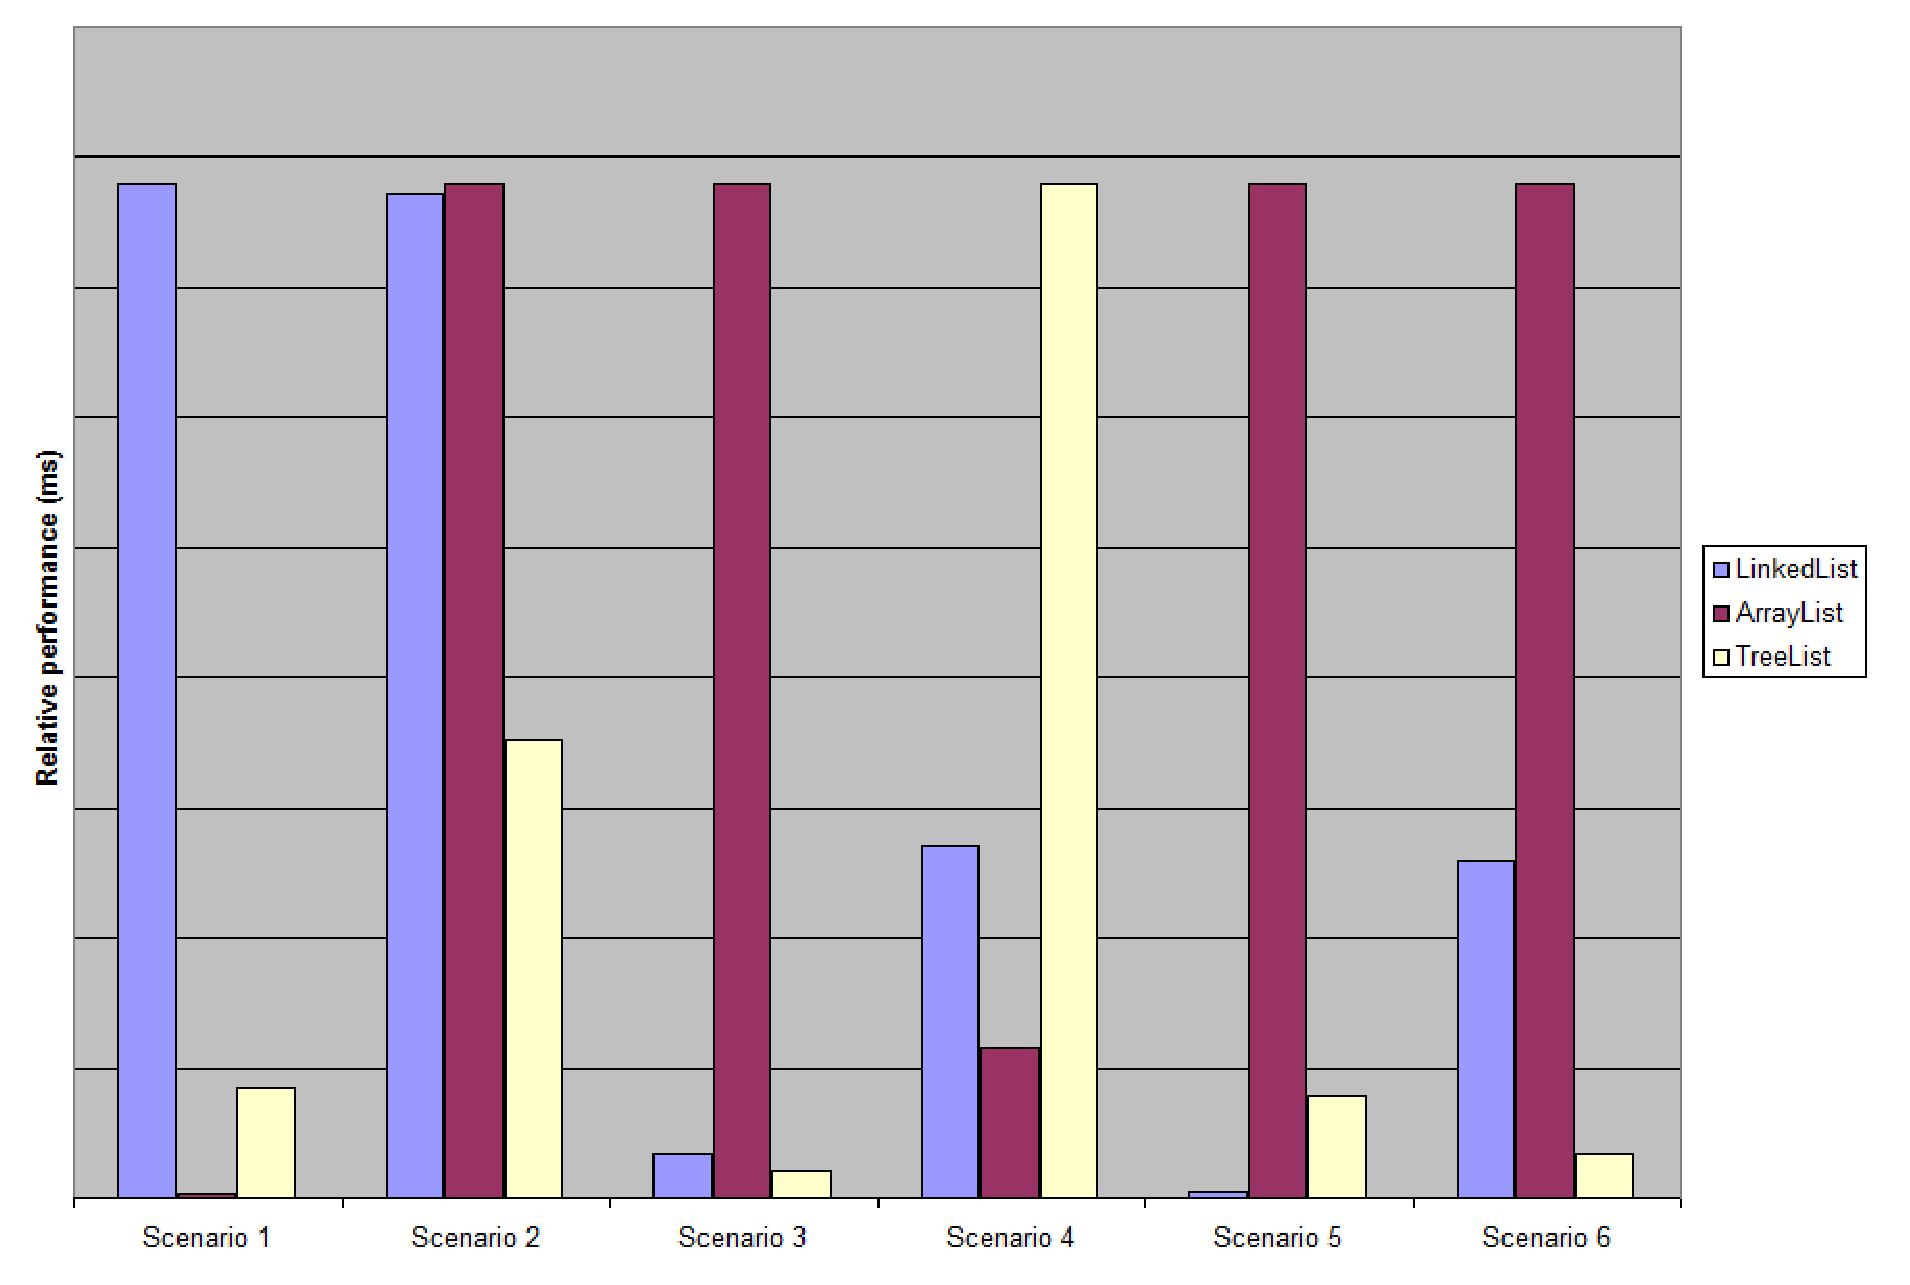
\includegraphics[scale=0.25]{scenarios.eps}
              \caption{Execution scenarios}
 \label{scen}
\end{figure}

As the number of the elements from the list grows, a proper data structure selection becomes more important. We depict in Figure \ref{perf}, for Scenario $1$, how the time needed for executing a usage scenario grows with the size of the list. 

\begin{figure}[h]
   \centering
          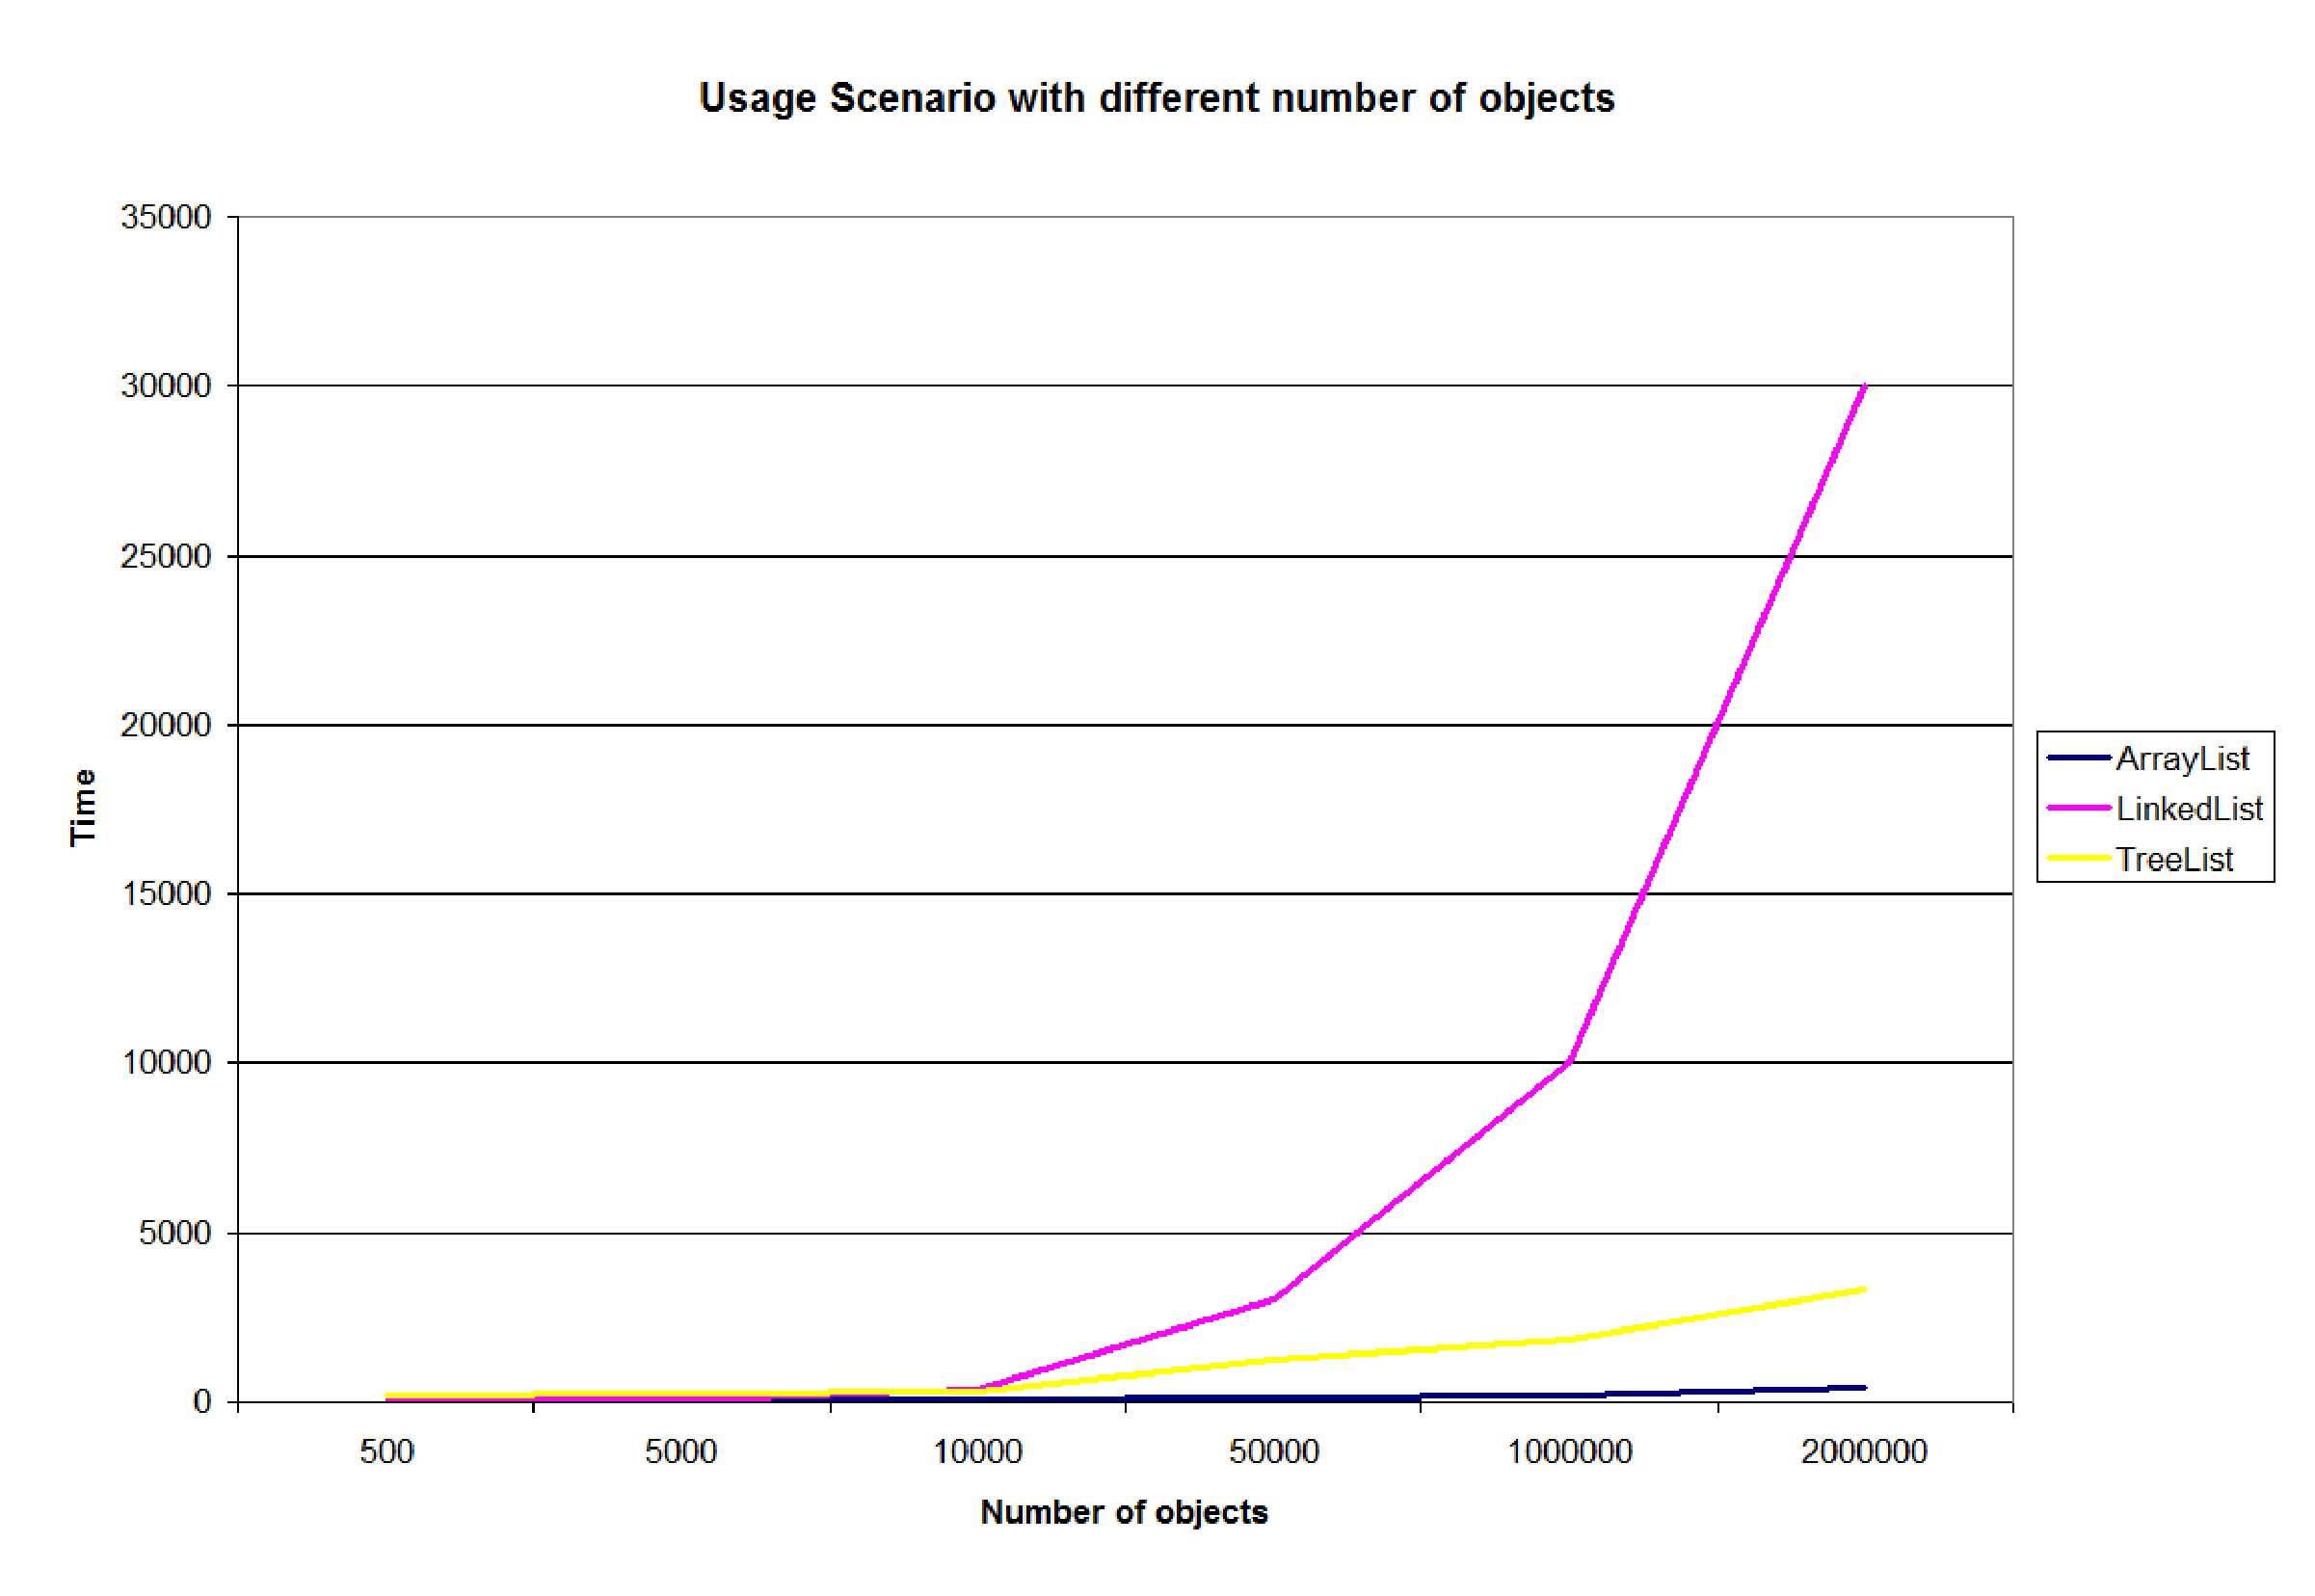
\includegraphics[scale=0.2]{performance.eps}
              \caption{Performance}
 \label{perf}
\end{figure}

The experiments described in this section confirms the importance of proper data structure selection and reveal the need for a dynamic decision according to the software system's actual usage scenario. 
  
\subsubsection{Related work for \emph{DRSP}}\label{rw}  

In this section we present several existing approaches for the problem of automatic selection of data repesentations. To our knowledge, so far, there are no existing machine learning approaches for the considered problem, and, moreover, there are no publicly available case studies for it. 

Low has introduced in \cite{Low} a method of choosing the most appropriate representation of a data structure based on data flow analysis, monitoring executions and user interrogations. The monitoring step uses a special compiler in order to acquire data about the number of executions of each statement in a program. Based on the above mentioned information, a selection algorithm will choose the most appropriate representation using a cost function. The criterion used for automatic selection is to minimize the expected space-time product for the execution of the resulting program. The selection process is static, i.e made at compile time, and uses an iterative technique similar to \emph{hill climbing}.

In \cite{29} and \cite{30}, Bik and Wijshoff  approach the problem of compiler optimization of sparse codes by automatic data structure selection at compile time - so the programmer does not have to deal with the matrix sparsity explicitly. Nevertheless the dense declared data structures which are actually sparse have to be annotated and the appropriate data representation is generated based on this information.

Schonberg et al present in \cite{31} an algorithm for automatic selection of data representation at compile time in the SETL programming language. In SETL, the objects are (dynamically) assigned appropriate abstract data types, algorithms being implemented without specifying any concrete data structure at all. The authors note that the problem of automatic data structure selection is a complex one because each particular data structure is usually more efficient for some operations and less efficient for others and they are choosing the best representation based on a static analysis of the way in which specific objects are used.

In \cite{lowrovner}, Low et al discuss about some techniques of automating the choice of data structure representation. They are conducting their experiments in an ALGOL-60 based programming language called SAIL and the paper is also focused on the automatic selection of associative data structures. In particular, the authors are looking for several alternate structures for storing triples in SAIL, using a static selection process. The compiler will choose the representation which minimizes a cost function, this cost function being influenced by both the amount of time and memory. The use of a data structure within the program is also influencing this choice, this information being collected by the compiler after performing a static analysis, from a monitoring phase (information like the frequency of each primitive operation) and also by user interaction (information about the size of certain data structures at a given time). 

Rovner presents methods for automatically selecting data structures for programs which use associative data in \cite{rovner}. A library of representations is described and model of associative data is defined based on the idea that classes of associations should be characterized in both terms of operations and properties of data. The process of automatic selection begins with a flow analysis in which the system determines the possible runtime values of item variables at their points of use in the program, and the possible associations that could exist at run-time. The representation selection is done based on a cost function which takes into consideration the memory consumption and execution time. 

Yellin focuses in \cite{Yellin} on dynamically choosing the implementation  of a component in order to provide optimized usage of resources. The proposed approach uses a mechanism to monitor the types of requests the component is receiving, and adaptively switches implementations for optimal application performance. An algorithm for choosing the most appropriate representation is given, but the algorithm is restricted to exactly two possible implementations of the component. The algorithm has been applied for solving the adaptive selection of data structure problem, but with the same restriction of having only two possible implementations.

A probabilistic approach to the problem of automatic selection of data representations based on Markov processes is proposed in \cite{chuang} by Chuang and Hwang. The selection is done at runtime, but the request sequence (operations performed on the ADT) has to be a priori known in form of a probabilistic description. The algorithm has a preprocessing phase for constructing the Markov process using some local heuristics.

 
\subsubsection{Support Vector Machines}\label{bck}

Predictive modelling \cite{geisser} is the process by which a model is created or chosen to try to best predict the probability of a certain outcome. From a machine learning perspective, predictive models are generated using supervised learning techniques \cite{Russell02Artificial}. 

Support Vector Machines (SVMs) \cite{svm} are a set of related supervised learning methods used for classification and regression. SVM is a classification technique based on statistical learning theory \cite{nello, smola} that was applied with great success in many challenging non-linear classification problems and on large data sets. The basic idea is that a SVM constructs a hyperplane or a set of hyperplanes in a high dimensional space, which can be further used for classification, regression, or other tasks. A decision hyperplane built by a SVM  optimally splits the training set, being a boundary between a set of objects having different class memberships \cite{wspsvm}. The optimal hyperplane can be distinguished by the maximum margin of separation between all training points and the hyperplane.

A SVM uses a nonlinear mapping to transform the original
training data into a higher dimension \cite{nello}. This is a promising
new method for the classification of both linear and non
linear data. Within this new dimension, it searches for
the linear optimal separating hyperplane that is, a
``decision boundary'' separating the tuples of one class
from another.

The advantages of the SVM method are as follows \cite{wspsvm}:

\begin{itemize}

\item They are highly accurate.

\item SVM have the ability to model complex nonlinear decision
boundaries.

\item SVM are less prone to over fitting than other models.

\item They provide a compact description of the learned
model.

\end{itemize}

SVM classifiers have a wide range of applications, being applied to a number of areas, including handwritten
digit recognition, object recognition, speech recognition \cite{speech}, predictions \cite{wspsvm}.






\subsection{Formal aspects}\label{tm}

Data structures \cite{adt} provide means to customize an abstract data type according to a given usage scenario. The volume of the processed data and the data access flow in the software application influence the selection of the most appropriate data structure for implementing a certain abstract data type. During the execution of the software application, the data flow and volume is fluctuating due to external factors (such as user interaction), that is why the data structure selection has to be dynamically adapted to the software system's execution context. This adaptation has to be made during the execution of the software application and it is hard or even impossible to predict by the software developer. Consequently, in our opinion, machine learning techniques would provide a better selection at runtime of the appropriate data structure for implementing a certain abstract data type.

In this section we will present our proposal of using supervised learning for dynamically selecting the implementation of an abstract data type from the software system, based on its execution context. For this purpose, a SVM model is proposed. In fact, selecting the most appropriate implementation of an abstract data type is equivalent to predicting, based on the execution
context, the type and the number of operations performed on the ADT, on a certain execution scenario.

Let $S=\{s_1, s_2, ..., s_n\}$ be an object oriented software system, where $s_i, 1 \le i \le n$ can be an application class, a method from a class or an attribute from a class.

We will consider that:

\begin{itemize}

\item $Class(S)=\{C_{1}, C_{2}, \dots , C_{l}\}$, $Class(S) \subset S$, is the set of applications classes of the software system $S$. 

\item Each application class $C_i$ ($1 \le i \le l$) is a set of methods and attributes, i.e., $C_i=\{m_{i1}, m_{i2}, \dots , m_{ip_{i}}, a_{i1}, a_{i2}, \dots , a_{ir_{i}} \}, \; 1 \le p_i \le n, \; 1 \le r_i \le n$, where $m_{ij}$ ($\forall j,\; 1 \le j \le p_i$) are methods  and $a_{ik}$ ($\forall k, \; 1 \le k \le r_i$) are attributes from $C_i$.

\item $Meth(S)= \displaystyle\bigcup_{i=1}^{l}\displaystyle\bigcup_{j=1}^{p_i}{m_{ij}}$, $Meth(S) \subset S$, is the set of methods from all the application classes of the software system $S$.

\item $Attr(S)= \displaystyle\bigcup_{i=1}^{l}\displaystyle\bigcup_{j=1}^{r_i}{a_{ij}}$, $Attr(S) \subset S$, is the set of attributes from the application classes of the software system $S$.

\end{itemize}

Based on the above notations, the software system $S$ can be defined as in Equation (\ref{sistem}):

\begin{equation}\label{sistem}
S=Class(S)\bigcup Meth(S) \bigcup Attr(S).
\end{equation}

Let us consider that $\mathcal{T}$ is an abstract data type having in its interface a set of operations $\mathcal{O}$ that can be performed on an instance of $\mathcal{T}$. We also consider a set $\mathcal{D}_\mathcal{T}=\{\mathcal{D}_1, \mathcal{D}_2, ... , \mathcal{D}_n\}$ of data structures that can be  used in the software system $S$ for implementing $\mathcal{T}$. If a given instance $c$ of a class $C \in Class(S)$ uses  $\mathcal{T}$, the selection of the appropriate data structure from $\mathcal{D}$ that has to be used for implementing (and instantiating) $\mathcal{T}$ depends on the states of the objects that are in a ``neighbourhood'' of object $c$. Intuitively, the classes that use directly or indirectly the $\mathcal{T}$ ADT influence the selection. 

In order to express the ``neighbourhood'' of an object, we define the \emph{distance} between any two classes from the software system. In our view, the \emph{distance} between two classes $C_i$ and $C_j$ expresses the degree to which class $C_i$ influences the behaviour of class $C_j$. 

In the following we will introduce several auxiliary definitions needed for a formal description of the notion of ``neighbourhood''.

\vspace{0.4cm}

\noindent
\begin{definition}\label{def_use}
{\it Let $c$ and $c^\prime$ be two objects which are instances of classes $C \in Class(S)$ and $C^\prime \in Class(S)$, respectively. We say that $c$ {\bf uses} $c^\prime$ if $c$ invokes a method from $c^\prime$ or $c^\prime$ invokes a method from $c$}.
\end{definition}


\noindent
\begin{definition}\label{def_usage}
{\it Let $c$ and $c^\prime$ be two objects which are instances of classes $C \in Class(S)$ and $C^\prime \in Class(S)$, respectively. The list $UC(c, c^\prime)=(c_1, c_2 \dots c_k)$ is called the {\bf usage chain} between $c$ and $c^\prime$ if $k \geq 2$, $c_i$ are instances of classes from $S$, $c_i$ {\bf uses} $c_{i+1}$ $\forall 1 \leq i \leq k-1$, $c=c_1$ and $c^\prime = c_k$ }.
\end{definition}

Intuitively, the \emph{usage chain} is similar with the idea of \emph{stack trace}. We denote by $\mathcal{UC}(c, c^\prime)$ the set of all existing \emph{usage chains} between objects $c$ and $c^\prime$. We mention that $\mathcal{UC}(c, c^\prime)$ can be empty if there is no \emph{usage chain} between the two objects. 

Considering the definitions above, we express the \emph{distance} between objects $c$ and $c^\prime$ as given in Equation (\ref{masura21}). By $|u|$ we denote the cardinality of set $u$.
\noindent
\begin{equation}\label{masura21}
d(c, c^\prime)=\left \{ \begin{array}{ll}
 0 & \;\;\emph{if} \; c=c^\prime\\
 \infty & \;\emph{if} \; \mathcal{UC}(c, c^\prime)=\emptyset\\
 min_{u \in \mathcal{UC}(c, c^\prime)}|u| & otherwise\\
 \end{array}, \right.
\end{equation}

In defining the \emph{distance} $d$ between two objects $c$ and $c^\prime$, as given in Equation (\ref{masura21}), we have started from the intuition that, as smaller the minimum length of an \emph{usage chain} between the objects is, as it is likely that the state of $c^\prime$ has a larger influence on $c$, so $c^\prime$ is ``closer'' to $c$ (the distance between $c$ and $c^\prime$ is smaller). It can be simply proved that $d$ is a semi-metric function.  

Now, the \emph{neighbourhood} of radius $\mathcal{R}$ of an object $o$, denoted by $\mathcal{N}_{\mathcal{R}}(c)$ can be defined as expressed in Equation (\ref{neighb}).

\begin{equation}\label{neighb}
\mathcal{N}_{\mathcal{R}}(c)= \{c^\prime | c^\prime \in InstClass(S), d(c, c^\prime) \leq \mathcal{R}  \}
\end{equation} 
where $\mathcal{R} \in N$ and $InstClass(S)=\{c| c \;is\;an\;instance\;of\;C \in Class(S)\}$ is the set of instances of the running software system $S$. 

It can be simply observed the following: 

\begin{itemize}

\item The neighbourhood of radius $0$ of any object $c$ consists only of itself, i.e, $\mathcal{N}_0(c)= \{c\}$.

\item If $\mathcal{R}$ is large enough, then the neighbourhood of radius $\mathcal{R}$ of any object $c$ consists of the entire system, i.e, $\mathcal{N}_{\mathcal{R}}(c)= InstClass(S)$.

\end{itemize}

Finally, the notion of \emph{execution context} of radius $\mathcal{R}$ for the abstract data type $\mathcal{T}$ will be introduced in Definition \ref{context}.     

\vspace{0.4cm}
\noindent
\begin{definition}\label{context}
{\bf Execution context} of $\mathcal{T}$. \\
{\it Let $c$ be an instance of a class $C_i \in Class(S)$ that uses $\mathcal{T}$. The {\bf execution context} of radius $\mathcal{R}$ of $\mathcal{T}$ represents the state of the objects from the neighborhood of $C_i$ at runtime, when $\mathcal{T}$ is initialized. Consequently, it is defined as a set $\mathcal{EC}_{\mathcal{R}}= \displaystyle\bigcup_{c_j \in \mathcal{N}_{\mathcal{R}}(c)}\{v_{j1}, v_{j2}, \dots , v_{jr_{j}} \}$, where $v_{j1}, v_{j2}, \dots , v_{jr_{j}}$, $\forall j$, represent the values of the attributes from object $c_j$.}  
\end{definition}


As we have shown in Section \ref{ex}, a ``static'' selection of the most suitable data structure from $\mathcal{D}_\mathcal{T}$ that has to be used for an efficient implementation of $\mathcal{D}$ is inappropriate and does not assure an efficient use of $\mathcal{T}$, as the volume of data manipulated by the implementation of $\mathcal{T}$ is unpredictable at the development stage. That is why a proper selection has to be done at runtime by analyzing the \emph{execution context}. 

In Definition \ref{customize} we will define the notion of \emph{suitable implementation} of $\mathcal{T}$ given a certain \emph{execution context}.

\begin{definition}\label{customize} \textbf{Most suitable implementation of $\mathcal{T}$ given the execution context $\mathcal{EC}_\mathcal{T}$.} \\
Let $\mathcal{T}$ be an abstract data type and $\mathcal{EC}_\mathcal{T}$ the execution context of $\mathcal{T}$ in a certain execution scenario. The most suitable implementation of $\mathcal{T}$ given the execution context $\mathcal{EC}_\mathcal{T}$ is the data structure $\mathcal{D}_i \in \mathcal{D}$ that provides an efficient implementation of $\mathcal{T}$ in the execution scenario, i.e. the time needed for performing the operations on $\mathcal{T}$ given the execution context $\mathcal{EC}_\mathcal{T}$ is minimized. 
\end{definition} 

In fact, the most proper implementation of $\mathcal{T}$  in a given execution scenario depends on the type and the number of operations from $\mathcal{O}$ that are performed on $\mathcal{T}$ during the execution. Thus, we can conclude that the problem of dynamically selecting the \emph{suitable implementation} of $\mathcal{T}$ is, in fact, the problem of predicting, based on the execution context, the type and the number of operations performed on $\mathcal{T}$ on a certain execution scenario.   

Considering the example given in Section \ref{ex}, the most suitable implementation of ADT \emph{Collection} in the execution context in which the collection has $10$ elements, and $2$ \textbf{searches} and $6$ \textbf{insertions} are performed on it is the \emph{list}.

\subsection{Methodology}
\label{sub:methodologysvm}
 
Let us consider, in the following, the theoretical model from Subsection \ref{tm}. Considering the issues described in the previous sections, for providing the most appropriate data structure for implementing an abstract data type $\mathcal{T}$ at runtime based on the system's \emph{execution context} we propose a \emph{supervised learning} \cite{mitchell} approach. 

In a software system $\mathcal{S}$, multiple occurences of $\mathcal{T}$ can be found. We mention that not all these occurences are subject for optimization, but only those that are considered to have a great impact on the system's performance. The software developer is responsible for selecting the locations in $S$ where optimization is needed. So, let us focus, in the following, on a single occurence of an abstract data type $\mathcal{T}$, for which $n$ possible implementations exist, i.e. $n$ data structures $\mathcal{D}_1, \mathcal{D}_2, ... , \mathcal{D}_n$.

In fact, the problem of identifying the most suitable implementation of $\mathcal{T}$, as illustrated in Definition \ref{customize}, can be viewed as a \emph{classification} \cite{mitchell} problem where each input is represented by an \emph{execution context}. The output for a given \emph{execution context} $\mathcal{EC}_\mathcal{T}$ is the index $i, 1 \leq i \leq n$ where $\mathcal{D}_i$ is the \emph{most suitable implementation of $\mathcal{T}$ given the execution context $\mathcal{EC}_\mathcal{T}$} (Definition \ref{customize}).

The classification process takes place in two phases that reflect the principles of a supervised learning algorithm: \emph{training} and \emph{testing}. As in any classification process, during the training a classification \emph{model} will be built, and during testing, the model built during the training will be applied for classifiying an unseen \emph{execution context} (input), i.e to predict the \emph{most suitable implementation} of $\mathcal{T}$ given the input \emph{execution context}. We propose a SVM classification model for the problem of identifying the most appropriate data reprezentation. 

For predicting the most \emph{suitable implementation} of a certain abstract data type $\mathcal{T}$, the following steps will be used:

\begin{enumerate}

\item Data Collection, Conversion and Pre-processing. 

\item Design of SVM Model.

\item Training.

\item Validation.

\item Testing.

\end{enumerate}

We mention that an innapropriate prediction does not impact the execution scenario of the software system. Even if the data structure selected for the implementation of the abstract data type $\mathcal{T}$ is not the most suitable one, the system execution is still successfull, even if  not the most efficient. We can imagine a classification model in which, if such an innacurate prediction is made, a feed-back is sent and the model is correspondingly adapted. The idea would be to send a \emph{reward} (\emph{reinforcement}) to the model, as in a \emph{reinforcement learning} \cite{sutton} based model.   

In the following we will briefly describe the above proposed steps. 

\subsubsection{Data collection, conversion and pre-processing}\label{col}

First, the software system $S$ is monitored during the execution of a set of scenarios that include the instantiation of the abstract data type $\mathcal{T}$. The result of this supervision performed by a software developer is a set of \emph{execution contexts}, as well as the type and the number of operations from $\mathcal{O}$ performed on $\mathcal{T}$ saved in a log file. 
The software developer will analyze the resulted log file and will decide, for each \emph{execution context} (input) , the \emph{most suitable implementation} for $\mathcal{T}$ given the \emph{execution context} (output). This decision will be based on computing the global computational complexity of the operations performed on $\mathcal{T}$ during the scenario given by the \emph{execution context} for each possible implementation of $\mathcal{D}_i$ of $\mathcal{T}$ and then selecting the implementation that minimizes the overall complexity.

This way, a data set consisting of (input, output) pairs is built. An input represents an \emph{execution context} $\mathcal{EC}_\mathcal{T}$ of the abstract data type $\mathcal{T}$ and the associated output represents the  the index $i, 1 \leq i \leq n$ where $\mathcal{D}_i$ is the \emph{most suitable implementation of $\mathcal{T}$ given the execution context $\mathcal{EC}_\mathcal{T}$} (Definition \ref{customize}).

The input data from the resulting data set (the \emph{execution contexts}) is now converted and pre-processed. 

First, the values of the attributes within an \emph{execution context} are converted to numerical values. This conversion is made as follows:

\begin{itemize}

\item An ordinal type attribute (integer, character, boolean, enumerated type) is converted to the ordinal position of the attribute value in its type domain.   

\item A numerical non-ordinal attribute (float, double), the actual value of the attribute remains unchanged.

\item For a string attribute or other user defined types, the corresponding numerical value is determined using a hash function \cite{Cormen09Introduction}. Such a hash function is available in most object-oriented programming languages. Even if two different attributes values can have the same hash value, the combination of all attributes values from the execution context may assure a uniqueness for the input data.    

\end{itemize} 
 
Then the input data is scaled to [0,1], and a statistical analysis is carried out in order to find a subset of attributes (from the \emph{execution contexts}) that are correlated with the target output.  The statistical analysis on the attributes from the \emph{execution contexts} is performed in order to reduce the dimensionality of the input data (the execution contexts), by eliminating attributes from the \emph{execution context} which do not influence the output value. 

To determine the dependencies between attributes and the target output, the Spearman's rank correlation coefficient \cite{spearman} is used. A Spearman correlation of $0$ between two variables $X$ and $Y$ indicates that there is no tendency for $Y$ to either increase or decrease when $X$ increases. A Spearman correlation of $1$ or $-1$ results when the two variables being compared are monotonically related, even if their relationship is not linear.  At the statistical analysis step we remove from the \emph{execution context} those attributes that have no significant influence on the target output, i.e are slightly correlated with it. A slight correlation is indicated by a value that is very close to $0$. Namely, an attribute $\mathcal{A}$ is removed from the \emph{execution context} if the correlation coefficient between $\mathcal{A}$ and the target output is less than a given threshold $\epsilon$ close to $0$. In our experiments, we have considered the threshold $\epsilon=10^{-1}$.

The data set preprocessed this way, denoted by $\mathcal{D}$, can now be used for building the classification model.

\subsubsection{The design of the SVM classification model}

SVMs use a technique known as the ``kernel trick'' to apply linear classification
techniques to non-linear classification problems. Using a Kernel function \cite{vapnik}, the data points from the input space are mapped into a higher dimensional space. Constructing (via the Kernel function) a separating hyperplane with maximum margin in the higher dimensional space yields a non-linear decision boundary in the input space separating the tuples of one class
from another.

The classification process takes place in two phases that reflect the principles of a supervised learning algorithm: \emph{training} and \emph{testing}. As in any classification process, during the training a classification \emph{model} will be built, and during testing, the model built during the training will be applied for clasifiying an unseen \emph{execution context} (input).

Therefore, the data set collected at step 1 has to be divided in two
parts: a part for \emph{training} and a part for \emph{testing}. The training part is divided
again in: a \emph{learning subset} used by the SVM algorithm in order to learn the
model that performs the class separation, and a \emph{validation subset} used in
order to optimise the values of the hyper parameters. The SVM model, which
is learnt in this manner, classifies the unseen \emph{execution contexts} from
the test set, which is disjoint to the training one.

In order to classify the \emph{execution contexts}, the SVM algorithm uses a kernel function. The parameters of the SVM
model (the penalty for miss-classification \emph{C} and the \emph{kernel parameters}) are
optimized on the validation set. A cross-validation framework is used in
order to avoid the overfitting problems. 

\subsubsection{Technical details}

In our current implementation, we have considered \emph{execution contexts} of radius $0$ (i.e. $\mathcal{R}=0$). This means that the execution context contains only the state of the object that uses the abstract data type $\mathcal{T}$ considered for optimisation.

For the monitored abstract data type $\mathcal{T}$ from the software application, a modified data structure implementation is used. This data structure implementation delegates all its methods to the actual data structure implementation, collects the state of the objects from the \emph{execution context} and writes the collected data into a log file. The modified data structure implementation has a reference to its container object (received as a constructor parameter) and uses it in order to determine the current state of the object.  

In the future we plan to extend the implementation in order to consider \emph{execution contexts} of arbitrary radius. For this, we need a more elaborate implementation in order to consider the \emph{usage chains} between objects. The \emph{usage chains} can be obtained by analysing the stack trace of the current execution. For obtaining the states of all objects from an \emph{usage chain}, references to the objects are needed. Using \emph{aspect oriented programming} \cite{kiczales97}, or instrumenting the software system classes (by using bytecode manipulation frameworks \cite{asm}) the needed references can be obtained.  

\section{Computational experiments} \label{compexp}

In this section we aim at evaluating the accuracy of the technique proposed in Section \ref{our}, i.e. the SVM classification model's prediction accuracy.

As there is no publicly available case study for the problem of automatic selection of data representations, nor a case study in the related literature that can be reproduced, we consider our own case studies. We describe in this section simulation results of applying
our classification approach to two selection problems that will be described in the following.

\subsection{SVM model}

From all the samples from $\mathcal{D}$ (obtained as indicated in Subsection \ref{col}), $\frac{2}{3}$ of them are considered for training the SVM
algorithm and $\frac{1}{3}$ of them for testing the classifier.
The C-SVM algorithm, provided by LIBSVM \cite{libsvm}, with a RBF kernel is
actually used in this experiment. It is not known beforehand which are the best values for the parameters of the SVM model ($C$ and $\gamma$), so some kind of model selection must be done. The optimisation of the hyper-parameters
is performed by a grid search method. A grid search makes repeated trials for each parameter across a specified interval using geometric steps.  For each combination of these
parameters, a 10-fold cross-validation is performed during the training phase,
the quality of a combination being computed as the average of the accuracy
rates estimated for each of the 10 divisions of the data set. 
We are using the following sequences for $C$ and $\gamma$:  $C=(2^{-5}, 2^{-3},..., 2^{15})$ and $\gamma=(2^{3},2^{1},...,2^{-15})$.

\emph{Cross-validation} is a popular technique for estimating the generalization error and there
are several interpretations \cite{wahba}. In $k$-fold cross-validation, the training data is randomly split
into $k$ mutually exclusive subsets (or folds) of approximately equal size. The SVM decision
rule is obtained by using $k$-1 subsets on training data and then tested on the subset left
out. This procedure is repeated $k$ times and in this manner each subset is used for testing
once. Averaging the test error over the $k$ trials gives a better estimate of the expected
generalization error.

Therefore, the best combination of parameters is indicated by the best average accuracy rate.

In order to obtain the accuracy of the model, considering the data set $\mathcal{D}$, the following cross-validation is used.

\begin{itemize}

\item  For a given number of episodes ($50$ in our experiment) repeat the following:

\begin{itemize}

\item $\frac{2}{3}$ randomly selected samples from $\mathcal{D}$ are used for training. Thus, for each training sample, the corresponding (pre-processed) \emph{execution context} with the associated output is provided to the SVM.  

\item The rest of $\frac{1}{3}$ samples from $\mathcal{D}$ are used for testing. After the training was completed, the SVM model is tested as follows. The \emph{execution context} within the testing sample is sent to the SVM. After receiving the \emph{execution context}, the SVM will predict the most appropriate output (the most \emph{suitable implementation} of the abstract data type $\mathcal{T}$ considered for optimization).     
\item The \emph{learning accuracy} on the current episode is computed as the number of accurate predictions divided by the number of tesing samples. 

\end{itemize}

\item The overall \emph{learning accuracy} of the SVM classification model is computed as the average of the learning accuracies over all episodes. 

\end{itemize}   

\subsection{First case study}\label{cs}

Starting from the data set given at \cite{forina}, we have simulated an experiment for selecting the most appropriate data structure for implementing the $List$ ADT. The considered data set consists of the results of a chemical analysis of wines grown in the same region in Italy but derived from  different cultivars. The analysis determined the quantities of $13$ constituents found in each types of wines. More details about this data set can be found at \cite{website:wine}.

In the proposed case study, we consider a $WineShop$ application that stores information about different wines and allows the user to locate wine shops according to different search criteria. In our simulation, we are focusing on the main class of the application, the class $Wine$, which models a type of wine by $13$ constituents given at \cite{website:wine}. This class has a method $getShops$ that returns a $List$ of shops where the current wine is available. For the $List$ ADT returned by $getShops$ method we aim at identifying the most suitable data structure for implementation.  As presented in Subsection \ref{exper}, three data structures for implementing a $List$ are considered: \textbf{vector} (dynamic array), \textbf{linked list} and \textbf{balanced search tree}. 

The $List$ of shops is used in three different usage scenarios:

\begin{enumerate}

\item [S1.] The $List$ of shops is presented to the user sorted according to different user selected criteria. In this scenario, the main operations performed on the $List$ are: \textbf{accessing} an element from a certain position and \textbf{updating} an element from a certain position. Consequently, the \textbf{dynamic array} data structure would be the most efficient implementation for the $List$ ADT.

\item [S2.] The $List$ of shops is presented to the user filtered according to different user selected criteria. In this scenario, the main operation performed on the $List$ is \textbf{removing} an element from a certain position. Consequently, the \textbf{balanced search tree} data structure would be the most efficient implementation for the $List$ ADT.

\item [S3.] The $List$ of shops is presented to the user by concatenating the shops lists from different wine types. In this scenario, the main operation is \textbf{adding} an element at the end of a list. Consequently, the \textbf{linked list} data structure would be the most efficient implementation for the $List$ ADT.

\end{enumerate}

In practice, the selection of most appropriate implementation of the $List$ is difficult, even impossible for a software developer, as it is hard to anticipate the data flow during the execution of the application. That is why we apply our supervised learning approach for a dynamic selection of the suitable implementing data structure of the $List$, according to the system's execution context. 

\subsubsection{Data collection and pre-processing}

The data set for evaluating the SVM classification model presented in Section \ref{our} consists of (input, output) samples collected and pre-processed as we have described in Subsection \ref{col}. An input represents an \emph{execution context} and the target output is the most suitable implementation for the $List$ ADT (\textbf{vector}, \textbf{linked list} or \textbf{balanced search tree}) within the input \emph{execution context}. The data set consists of $178$ samples. 

After data was scaled, a statistical analysis is carried out in order to find a subset of attributes that are correlated with the target output. To determine the dependencies between attributes and the target output, the Spearman's rank correlation coefficient \cite{spearman} is used.   

Figure \ref{sper} shows the correlations between the attributes from the $Wine$ class (the current \emph{execution context} for the $List$ of shops) and the target output (the most suitable data structure for implementing the $List$ of shops) computed using the Spearman's rank correlation coefficient \cite{spearman}. 

\begin{figure}
   \centering
       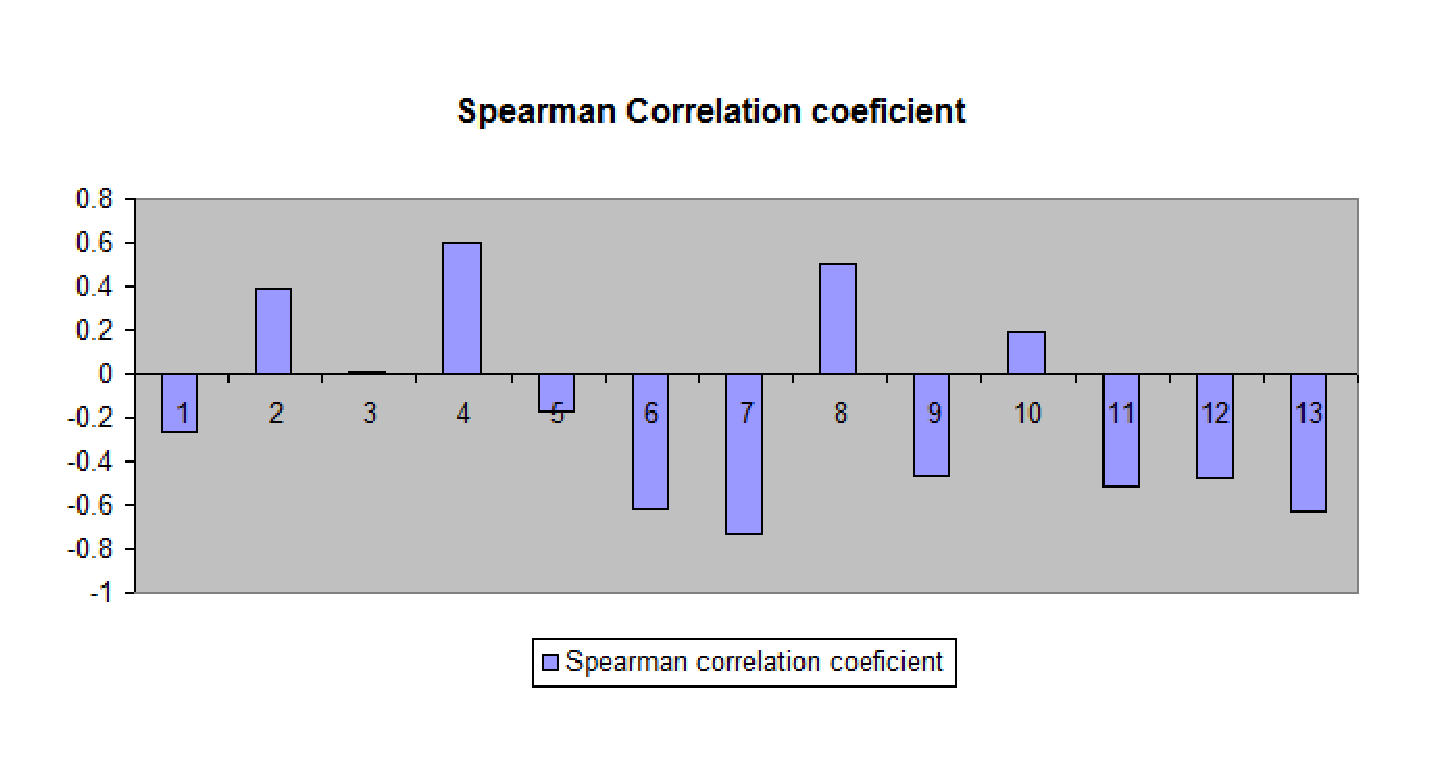
\includegraphics[scale=0.28]{cor.eps}
              \caption{Spearman correlation}
 \label{sper}
\end{figure}

After an analysis of the correlation between the attributes from the $Wine$ class (current \emph{execution context} for the $List$ of shops) and the target output, considering the value $10^{-1}$ for the threshold $\epsilon$ (Subsection \ref{col}), we can conclude that attribute \textbf{3} is slightly correlated with the target output (its correlation with the output is $0.01403$). Consequently, we can consider that the above mentioned attribute has no significant influence on the target output. Thus, after the performed statistical analysis, there are $12$ attributes identified to be relevant for our classification task (the attributes from the $Wine$ class excepting attribute \textbf{3}). 

\subsubsection{Results}

The \emph{learning accuracies} obtained for each episode are given in Figure \ref{sprec1}. An overall \emph{learning acuracy} of $0.9625$ was obtained.
As we can see in Figure \ref{sprec1}, the results are stable, a standard deviation of $0.033071891$ on the classification accuracies was obtained. The low value of the standard deviation indicates a good precision of our approach.  
  
\begin{figure}
   \centering
       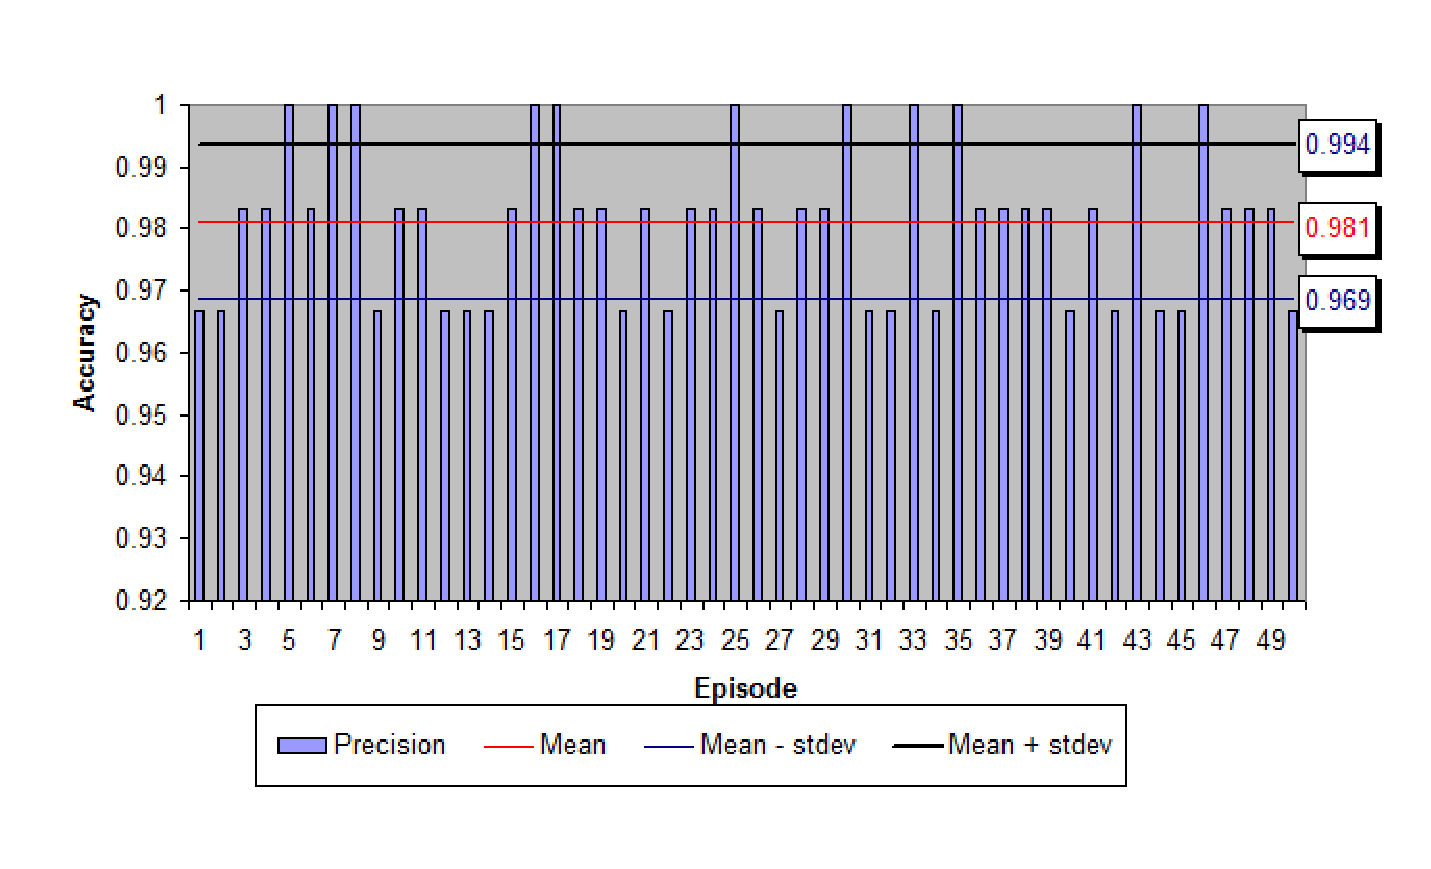
\includegraphics[scale=0.28]{prec.eps}
              \caption{Results for the first case study}
 \label{sprec1}
\end{figure}

\subsection{Second case study}\label{cs}

We will consider a real software system as a case study for evaluating the learning accuracy of the SVM. It is a DICOM (\emph{Digital Imaging and Communications in Medicine}) \cite{dicom} and HL7 (\emph{Health Level 7}) \cite{hl7} compliant PACS (\emph{Picture Archiving and Communications System}) system, facilitating medical images management, offering  quick access to radiological images, and making the diagnosing process easier. The analyzed application is a large distributed system, consisting of several subsystems in form of stand-alone and web-based applications. We have considered as our case study one of the subsystems from this application.  The analyzed subsystem is a stand-alone Java application used by physicians in order to interpret radiological images. The application fetches clinical images from an image server (using DICOM protocol) or from the local file system (using DICOM files), displays them, and offers various tools to manage radiological images. 

Radiological images are produced by medical devices called modalities. The modalities generate multiple related images, organized in series. 

Let us consider the Java source code fragment presented below, extracted from the analyzed software system, where \textbf{ImageSeries} class represents an image serie acquired by a medical device for a given human body part. The medical device sends additional information which characterize: the performed medical procedure ($code$, $description$), technical aspects related to the device ($thickness$, $frecquency$, \emph{repetition time}), aspects related to the patient ($bodyPart$, $localizer$), etc. Some relevant aspects are captured in the \textbf{ImageSeries} attributes. In practice, the size of the list of images contained in an image serie significantly vary. That is why we apply our approach for dynamically configuring the image list from an image serie, according to the execution context.

\begin{footnotesize}
 \begin{verbatim}
public class ImageSeries {
 	   
   private String modality;
	   private String code;
	   private String bodyPart;
	   private String manuf;
	   private String model;
	   private String description;
	   private String localizer;
	   private float thickness;
	   private float frecquency;
	   private int repetitionTime;
13.private List<Image> images;
	   private String UID;

	  public Series(DicomObject d) {
		    UID = 
		     d.getString(Tag.SeriesInstanceUID);
		    bodyPart = 
		     d.getString(Tag.BodyPartExamined);
		    modality = 
		     d.getString(Tag.Modality);
		    localizer = d.getString(Tag.ImageType);
		    manuf = d.getString(Tag.Manufacturer);
		    model = 
		     d.getString(Tag.ManufacturerModelName);
20.		images = new ArrayList<Image>();
		    ....  
	  }

	  public void setCode(String code) {
		    this.code = code;
	  }

	  public void addImages(Image img) {
		    images.add(img);
	  }

	  public boolean isLocalizer() {
		    if (imgType == null) {
			    return false;
		    }
		    return imgType.contains("LOCALIZER");
	  }

	  public Modality getModality() {
		    return Modality.valueOf(modality);
	  }

	  public String getBodyPart() {
		    return bodyPart;
	  }

	  public String getManuf() {
		    return manuf;
	  }

	  public String getModel() {
		    return model;
	  }

	  public String getProcT() {
		    return code;
	  }

	  public String getDescr() {
		    return description;
	  }

	  public String getUID() {
		    return UID;
	  }

	  public int getNoOfImages() {
		    return images.size();
	  }

	  public boolean equals(Object o) {
		    return ((Series) o).UID.equals(UID);
	  }
	  .....
}
\end{verbatim} 
\end{footnotesize}

For the $images$ attribute in line 13 from the source code below, the most suitable data structure implementation has to be chosen at runtime (line 20).  As presented in Subsection \ref{exper}, three data structures for implementing a $List$ are considered: \textbf{vector} (dynamic array) ($ArrayList$ class from Java SDK), \textbf{linked list} ($LinkedList$ class from Java SDK) and \textbf{balanced search tree} ($TreeList$ class from Apache Collection API \cite{apache}). 

The $List$ of images is used in three different usage scenarios:

\begin{enumerate}

\item [S1.] The $List$ of images are sorted according to different criteria (position of the image relative to the patient, image acquisition time, etc). This operation is required in order to provide the physician a consistent presentation of the images list. In this scenario, the main operations performed on the $List$ are: \textbf{accessing} an element from a certain position and \textbf{updating} an element from a certain position. Consequently, the \textbf{dynamic array} data structure would be the most efficient implementation for the $List$ ADT.

\item [S2.] The $List$ of images is filtered according to different criteria (echo time, constrast agent). This operation is required in particular medical procedure which require the acquisition of multiple images from the same body part, for example head CT performed twice: once without any contrast substance and second with a contrast agent. In this scenario, the main operation performed on the $List$ is \textbf{removing} an element from a certain position. Consequently, the \textbf{balanced search tree} data structure would be the most efficient implementation for the $List$ ADT.

\item [S3.] The $List$ of images is created by the physician through an iterative step by step process. For example, the physician selects relevant images from source series and creates a new image serie with the relevant images. In this scenario, the main operation is \textbf{adding} an element at the begining/end of a list. Consequently, the \textbf{linked list} data structure would be the most efficient implementation for the $List$ ADT.

\end{enumerate}

In practice, the selection of the most appropriate implementation of the $List$ of images is difficult, as it is hard to anticipate the usage scenario of the image serie object at its instantiation time. That is why we apply our supervised learning approach for a dynamic selection of the suitable implementing data structure of the $List$, according to the system's execution context. 

\subsubsection{Data collection and pre-processing}

We have used for evaluation a set of $96$ image series samples which were obtained from publicly available DICOM image files \cite{im1, im2, im3, im4, im5}. The images are real images from real patients, but anonymized for confidentiality reasons. For managing the DICOM image files, an open source implementation of the DICOM standard was used \cite{im6}.

The data set for evaluating the SVM classification model presented in Section \ref{our} consists of (input, output) samples collected and pre-processed as we have described in Subsection \ref{col}. An input represents an \emph{execution context} and the target output is the most suitable implementation for the $List$ ADT (\textbf{vector}, \textbf{linked list} or \textbf{balanced search tree}) within the input \emph{execution context}. 

After data was scaled, a statistical analysis is carried out in order to find a subset of attributes that are correlated with the target output. To determine the dependencies between attributes and the target output, the Spearman's rank correlation coefficient \cite{spearman} is used.   


Figure \ref{cor} shows the correlations between the attributes from the $ImageSeries$ class (the current \emph{execution context} of the $images$ List) and the target output (the most suitable data structure for the $images$ List implementation) computed using the Spearman's rank correlation coefficient \cite{spearman}. 

\noindent\begin{figure}[h]
   \centering
       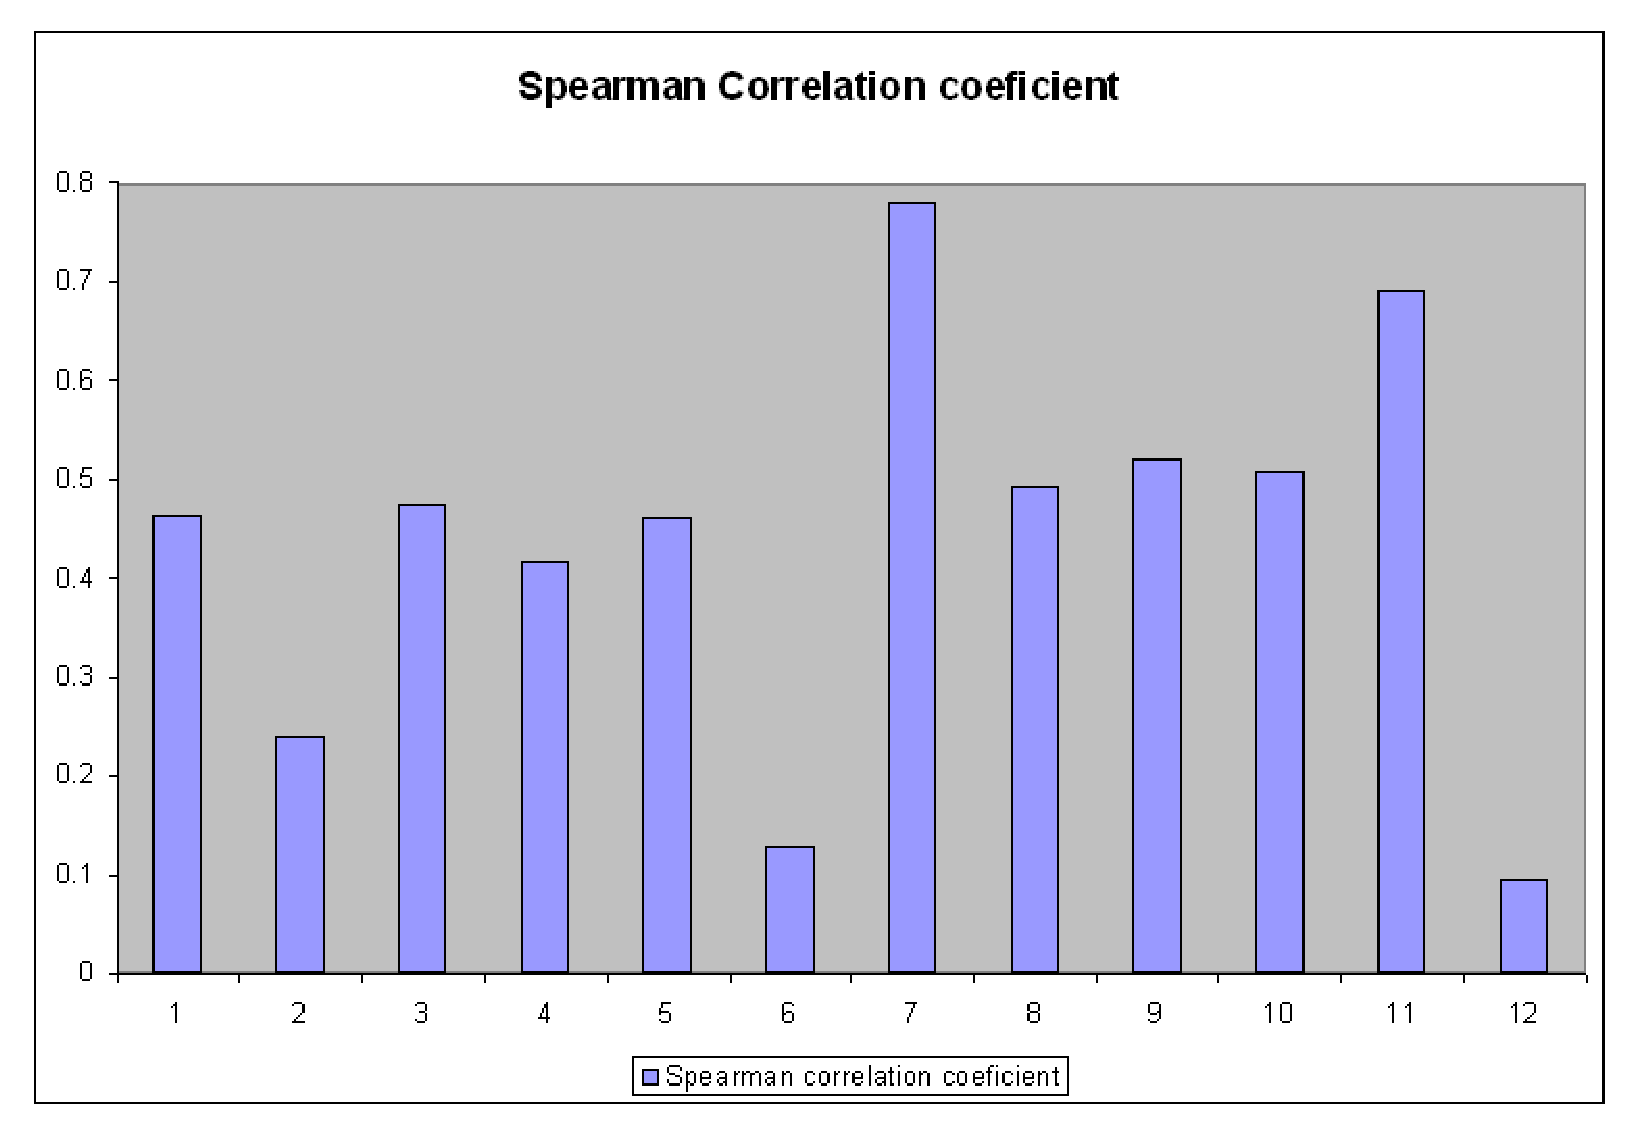
\includegraphics[scale=0.28]{cor2.eps}
              \caption{Spearman correlation}
 \label{cor}
\end{figure}

After an analysis of the correlation between the attributes from the $ImageSeries$ class (current \emph{execution context} for the $images$ list) and the target output, considering the value $10^{-1}$ for the threshold $\epsilon$ (Subsection \ref{col}), we can conclude that attribute \textbf{12} (\textbf{UID}) is slightly correlated with the target output (its correlation with the output is $0.09527$). Consequently, we can consider that the above mentioned attribute has no significant influence on the target output. Thus, after the performed statistical analysis, there are $11$ attributes identified to be relevant for our classification task (the attributes from the $ImageSeries$ class excepting $UID$ attribute). 

\subsubsection{Results}

The \emph{learning accuracies} obtained for each episode are given in Figure \ref{sprec2}. An overall \emph{learning acuracy} of $0.941875$ was obtained. As we can see in Figure \ref{sprec2}, the results are stable, a standard deviation of $0.040024407
$ on the classification accuracies was obtained. The low value of the standard deviation indicates a good precision of the proposed approach.  
  
\begin{figure}[h]
   \centering
       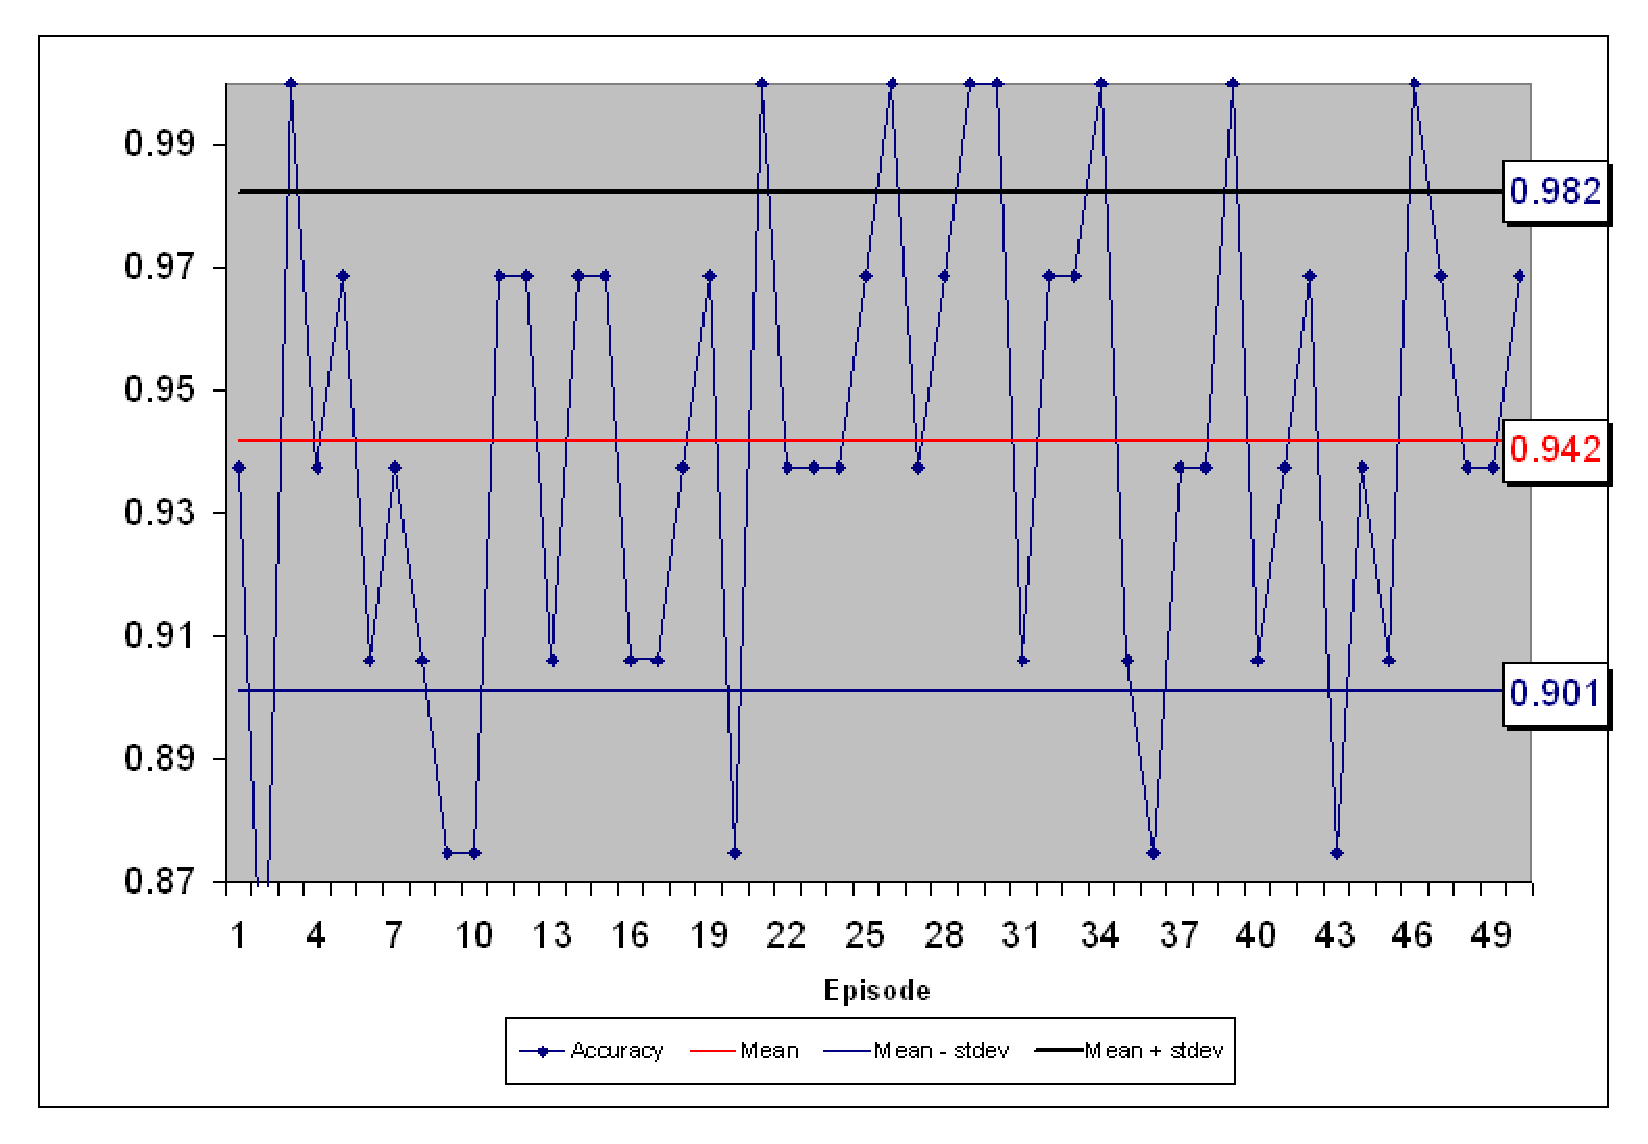
\includegraphics[scale=0.28]{prec2.eps}
              \caption{Results for the second case study}
 \label{sprec2}
\end{figure}


\subsection{Discussion}\label{dis}

Considering the experimental results presented in Section \ref{compexp}, we can conclude that our approach provides optimized data structure selection and reduces the computational time by selecting the data structure implementation which provides a minimum overall complexity for the operations performed on a certain abstract data type on a given execution scenario.

We mention that the accuracy of the prediction process may depend on the radius $\mathcal{R}$ of the \emph{execution context}. In our opinion, choosing a larger value for $\mathcal{R}$ may increase the accuracy of the predicted customization parameters values.  
However, increasing the value for $\mathcal{R}$ leads to larger \emph{execution contexts}, and, consequently, to larger computational complexity. The most appropriate value for $\mathcal{R}$ may depend on the domain and complexity of the considered software system.

The results obtained for automatic data selection using supervised learning are promising.  Considering the results presented in Section \ref{compexp}, we can conclude that the approach introduced in this paper for a dynamic selection of data representations has the following advantages:

\begin{itemize}

\item It is general, as it can be used for determining the appropriate \emph{implementation} for any abstract data type, and with arbitrary number of data structures that can be chosen for implementing the ADT.   

\item It reduces the computational time by selecting the data structure implementation which provides a minimum overall complexity for the operations performed on a certain abstract data type on a given execution scenario. Consequently, it increases the efficiency of the software system during its evolution.

\item It is scalable, as even if the considered software system is large, the abstract data types optimisation depends on the radius $\mathcal{R}$ of the \emph{execution context}. The size of the execution context does not depend on the size of the software system.

\end{itemize}

However, the main drawback of our approach is that it is hard to supervise the learning process, as the supervision of an expert software developer is required for inspecting the collected execution contexts. That is why, in the future, we will investigate other learning techniques for solving the cosidered problem, i.e. reinforcement learning \cite{sutton} and unsupervised learning \cite{mitchell}. 

      
\section{Comparison to related work}\label{sec:cmpsvm}


In this section we aim at providing a brief comparison of our approach with the existing approaches for the problem of automatic selection of data representations presented in Section \ref{rw}. 

Compared to the approaches from \cite{29, 30, 31, Low, lowrovner, rovner} which are based on a static analysis, the main advantage of our supervised learning based approach for data structures selection is that it is dynamic, i.e is made at runtime, not at compile time. As we have presented in Section \ref{mot}, a dynamic selection is more accurate than a static one. 

Even if the approach from \cite{Yellin} is dynamic, our approach is more general than it, as it can be used for an arbitrary number of ADTs implementations.    

A more detailed comparison with the techniques from \cite{29, 30, 31, Low, lowrovner, rovner, Yellin} can not be made, as the case studies used in experiments are not publicly available.  

The main difference between our approach and to the one from \cite{chuang} is that the request sequence does not have to be a priori known, it will be dynamically predicted. This is a main advantage, because, as we have indicated in Section \ref{mot}, the data access patterns are highly variant, or even unpredictable and can not be statically determined.  





\section{Conclusions and future work}\label{conc}

In this chapter we have presented our model for dynamically selecting the most suitable implementation of an abstract data type from a software application based on the system's execution context. For predicting, at runtime, the most appropriate data representation, a neural network and a support vector machine classification model were used. We have also illustrated the accuracy of both proposed approaches on case studies.

Considering the results presented in Section \ref{exp} and in Section \ref{compexp}, we can conclude that the approaches introduced in this paper for a dynamic selection of data representations have the following advantages:

\begin{itemize}

\item They are general, as they can be used for determining the appropriate \emph{implementation} for any abstract data type, and with arbitrary number of data structures that can be chosen for implementing the ADT.

\item They reduce the computational time by selecting the data structure implementation which provides a minimum overall complexity for the operations performed on a certain abstract data type on a given execution scenario. Consequently the efficiency of the software system during its evolution is increased.

\item They are is scalable, as even if the considered software system is large, the abstract data types are locally optimized, considering only the current execution context. The size of the execution context does not depend on the size of the software system (as shown in Section~\ref{tm}).

\end{itemize}

However, the main drawback of both approaches is that it is hard to supervise the learning process, as the supervision of an expert software developer is required for inspecting the collected execution contexts.

Further work will be focused on:

\begin{itemize}

\item Improving the proposed classification model by adding to it the capability to adapt itself using a feed-back received when inappropriate data representations are selected.

\item Applying other machine learning techniques  \cite{tezel,zhu} , self-organizing feature maps  \cite{koh}, or other modelling techniques  \cite{raykar,nguyen,takacs}   for solving the problem of automatic selection of data representations during the execution of a software system.

\item Studying the applicability of other learning techniques, like semi-supervised learning \cite{zhou} or reinforcement learning  \cite{sutton} in order to avoid as much as possible the supervision during the training process.

\item Evaluating our approach on other case studies and real software systems.

\end{itemize}

